\documentclass[a4paper]{report}
\usepackage[utf8]{inputenc}
\usepackage[T1]{fontenc}
\usepackage{RJournal}
\usepackage{amsmath,amssymb,array}
\usepackage{booktabs}


% tightlist command for lists without linebreak
\providecommand{\tightlist}{%
  \setlength{\itemsep}{0pt}\setlength{\parskip}{0pt}}

\usepackage{longtable}

% Always define CSL refs as bib entries are contained in separate doc
% Pandoc citation processing
\newlength{\cslhangindent}
\setlength{\cslhangindent}{1.5em}
\newlength{\csllabelwidth}
\setlength{\csllabelwidth}{3em}
\newlength{\cslentryspacingunit} % times entry-spacing
\setlength{\cslentryspacingunit}{\parskip}
% for Pandoc 2.8 to 2.10.1
\newenvironment{cslreferences}%
  {}%
  {\par}
% For Pandoc 2.11+
\newenvironment{CSLReferences}[2] % #1 hanging-ident, #2 entry spacing
 {% don't indent paragraphs
  \setlength{\parindent}{0pt}
  % turn on hanging indent if param 1 is 1
  \ifodd #1
  \let\oldpar\par
  \def\par{\hangindent=\cslhangindent\oldpar}
  \fi
  % set entry spacing
  \setlength{\parskip}{#2\cslentryspacingunit}
 }%
 {}
\usepackage{calc}
\newcommand{\CSLBlock}[1]{#1\hfill\break}
\newcommand{\CSLLeftMargin}[1]{\parbox[t]{\csllabelwidth}{#1}}
\newcommand{\CSLRightInline}[1]{\parbox[t]{\linewidth - \csllabelwidth}{#1}\break}
\newcommand{\CSLIndent}[1]{\hspace{\cslhangindent}#1}


\usepackage[most]{tcolorbox}
\usepackage{booktabs}
\usepackage{bm, amsmath}
\usepackage{array}
\usepackage{multirow}
\usepackage{wrapfig}
\usepackage{float}
\usepackage{colortbl}
\usepackage{xcolor}
\usepackage{longtable}
\usepackage{tabu}
\usepackage{adjustbox}
\usepackage{threeparttable}
\usepackage{makecell}
\def\greentick{
\includegraphics[scale=0.05]{figures/green_tick.png}}
\def\redcross{
\includegraphics[scale=0.05]{figures/red_cross.png}}
\newtcolorbox{blackbox}[1]{colback=white, colframe=black, coltext=black, boxsep=1.5pt, arc=4pt, before=\centering, title=#1}
\newenvironment{cols}[1][]{}{} \newenvironment{col}[1]{\begin{minipage}{#1}\ignorespaces}{\end{minipage} \ifhmode\unskip\fi
\aftergroup\useignorespacesandallpars} \def\useignorespacesandallpars#1\ignorespaces\fi{#1\fi\ignorespacesandallpars}


\begin{document}


%% do not edit, for illustration only
\sectionhead{Contributed research article}
\volume{15}
\volnumber{2}
\year{2023}
\month{June}
\setcounter{page}{56}

\begin{article}
  % !TeX root = RJwrapper.tex
\title{Gaussian Mixture Models in R}


\author{by Bastien Chassagnol, Antoine Bichat, Cheïma Boudjeniba, Pierre-Henri Wuillemin, Mickaël Guedj, David Gohel, Gregory Nuel, and Etienne Becht}

\maketitle

\abstract{%
Gaussian mixture models (GMMs) are widely used for modelling stochastic problems. Indeed, a wide diversity of packages have been developed in R. However, no recent review describing the main features offered by these packages and comparing their performances has been performed. In this article, we first introduce GMMs and the EM algorithm used to retrieve the parameters of the model and analyse the main features implemented among seven of the most widely used R packages. We then empirically compare their statistical and computational performances in relation with the choice of the initialisation algorithm and the complexity of the mixture. We demonstrate that the best estimation with well-separated components or with a small number of components with distinguishable modes is obtained with REBMIX initialisation, implemented in the \href{https://CRAN.R-project.org/package=rebmix}{rebmix} package, while the best estimation with highly overlapping components is obtained with \emph{k}-means or random initialisation. Importantly, we show that implementation details in the EM algorithm yield differences in the parameters' estimation. Especially, packages \href{https://CRAN.R-project.org/package=mixtools}{mixtools} (Young et al.~2020) and \href{https://CRAN.R-project.org/package=Rmixmod}{Rmixmod} (Langrognet et al.~2021) estimate the parameters of the mixture with smaller bias, while the RMSE and variability of the estimates is smaller with packages \href{https://CRAN.R-project.org/package=bgmm}{bgmm} (Ewa Szczurek 2021) , \href{https://CRAN.R-project.org/package=EMCluster}{EMCluster} (W.-C. Chen and Maitra 2022) , \href{https://CRAN.R-project.org/package=GMKMcharlie}{GMKMcharlie} (Liu 2021), \href{https://CRAN.R-project.org/package=flexmix}{flexmix} (Gruen and Leisch 2022) and \href{https://CRAN.R-project.org/package=mclust}{mclust} (Fraley, Raftery, and Scrucca 2022). The comparison of these packages provides R users with useful recommendations for improving the computational and statistical performance of their clustering and for identifying common deficiencies. Additionally, we propose several improvements in the development of a future, unified mixture model package.
}

\hypertarget{introduction-to-mixture-modelling}{%
\section{Introduction to Mixture modelling}\label{introduction-to-mixture-modelling}}

Formally, let's consider a pair of random variables \((X,S)\) with \(S \in \{1, \ldots, k\}\) a discrete variable and designing
the component identity of each observation. When observed, \(S\) is
generally denoted as the labels of the individual observations. \(k\) is
the number of mixture \emph{components}. Then, the density distribution of
\(X\) is given in Equation \eqref{eq:1}:

\begin{equation}
\begin{split}
f_\theta(X) &= \sum_S f_\theta (X, S) \\
&= \sum_{j=1}^k p_j f_{\zeta j}(X), \quad X\in\mathbb{R}
\end{split}
\label{eq:1}
\end{equation}

where \(\theta = (p, \zeta) = (p_1, \ldots, p_k, \zeta_1, \ldots, \zeta_k)\)
denotes the parameters of the model: \(p_j\) is the proportion of
component \(j\) and \(\zeta_j\) represents the parameters of the density
distribution followed by component \(j\). In addition, since \(S\) is a categorical variable parametrized by \(p\), the prior weights must enforce the unit simplex constraint (Equation \eqref{eq:2}):

\begin{equation}
\begin{cases}
p_j \ge 0 \quad \forall j \in \{1, \ldots, k \}\\
\sum_{j=1}^k p_j =1
\end{cases}
\label{eq:2}
\end{equation}

In terms of applications, mixture models can be used to achieve the
following goals:

\begin{itemize}
\tightlist
\item
  \emph{Clustering}: hard clustering consists in determining a complete
  partition of the \(n\) observations \(x_{1:n}\) into \(k\) disjoint
  non-empty subsets. In the context of \emph{mixture model-based
  clustering}, this is done by assigning each observation \(i\) to the
  cluster \(\hat{s_i}=\arg \max_j \eta_{i} (j)\) that maximises the
  posterior distribution (MAP) (see Equation
  \eqref{eq:posteriori}):
\end{itemize}

\begin{equation}
        \eta_{i} (j) := \mathbb{P}_{\theta} (S_i=j |X_i=x_i)
    \label{eq:posteriori}
\end{equation}

\begin{itemize}
\tightlist
\item
  \emph{Prediction}: the purpose is to predict a response variable \(Y\) from
  an explanatory variable \(X\). The dependent variable \(Y\) can either
  be discrete, taking values in classes \(\{1, \ldots, G\}\)
  (\emph{classification} task) or continuous (\emph{regression} task). In this
  paper, we do not extensively discuss application of mixture models to regression purposes but refer the reader
  to Bouveyron and Girard (2009) for mixture classification and
  Shimizu and Kaneko (2020) for mixtures of regression models.
\end{itemize}

In section \protect\hyperlink{univariate-and-multivariate-gaussian-distributions-in-the-context-of-mixture-models}{Univariate and multivariate Gaussian distributions in the context of mixture models}, we describe the most
commonly used family, the Gaussian Mixture Model (GMM). We then present
the MLE estimation of the parameters of a GMM, introducing the classic
EM algorithm in section \protect\hyperlink{parameter-estimation-in-finite-mixtures-models}{Parameter estimation in finite mixtures models}. Finally, we introduce bootstrap methods used to evaluate the
quality of the estimation and metrics used for the selection of the best
model in respectively appendices \emph{Derivation of confidence intervals in GMMs} and \emph{Model selection}.

\hypertarget{univariate-and-multivariate-gaussian-distributions-in-the-context-of-mixture-models}{%
\subsection{Univariate and multivariate Gaussian distributions in the context of mixture models}\label{univariate-and-multivariate-gaussian-distributions-in-the-context-of-mixture-models}}

We focus our study on the finite Gaussian mixture models (GMM) in which we
suppose that each of the \(k\) components follows a Gaussian
distribution.

We recall below the definition of the Gaussian
distribution in both univariate and multivariate context. In the finite univariate Gaussian mixture model, the distribution of
each component \(f_{\zeta j}(X)\) is given by the following univariate
Gaussian p.d.f. (probability density function) (Equation
\eqref{eq:gaussian-dist}):

\begin{equation}
f_{\zeta j}(X=x)=\varphi_{\zeta_j}(x | \mu_j, \sigma_j):=\frac{1}{\sqrt{2\pi} \sigma_j} \exp^{- \frac{(x - \mu_j)^2}{2 \sigma_j^2}}
\label{eq:gaussian-dist}
\end{equation} which we note: \(X \sim \mathcal{N}(\mu_j, \sigma_j)\).

In the univariate case, the parameters to be inferred from each
component, \(\zeta_j\), are: \(\mu_j\), the \emph{location} parameter (equal to
the mean of the distribution) and \(\sigma_j\), the \emph{scale} parameter
(equal to the standard deviation of the distribution with a Gaussian distribution).

Following parsimonious parametrisations with respect to univariate GMMs
are often considered:

\begin{itemize}
\item
  \emph{homoscedascity}: variance is considered equal for all components,
  \(\sigma_j = \sigma, \forall j \in \{1, \ldots, k \}\), as opposed to
  heteroscedascity where each sub-population has its unique
  variability.
\item
  \emph{equi-proportion} among all mixtures:
  \(p_j = \frac{1}{k} \quad j \in \{ 1, \ldots, k\}\) \footnote{A rarer constraint considered implies to enforce a linear
    constraint over the clusters' means, of the following general form:
    \(\sum_{j=1}^k a_j \mu_j=0\), with \(\{a_1, \ldots, a_k\}\). For
    instance, the R package \pkg{epigenomix} considers a \(k=3\) component
    mixture in the context of transcriptomic (differential analyses) and
    epigenetic (histone modification) to automatically identify
    undifferentiated, over and under-expressed genes between case and
    control samples. A common constraint then is to enforce the
    distribution of fold changes corresponding to the undifferentiated
    expressed genes to have a distribution centred on 0. Combining
    equality of means and equality of variances is irrelevant, as the
    model is then degenerate. Additionally, setting constraints on the
    means makes the estimation of the parameters challenging, as
    detailed in Appendix \emph{Extensions of the EM algorithm to overcome its limitations}.}
\end{itemize}

In the finite multivariate Gaussian mixture model, the distribution \(f_{\zeta j}(\boldsymbol{X})\) of each component \(j\), where
\(\boldsymbol{X} \in \mathbb{R}^D =(X_1, \ldots, X_D)^\top\) is a multivariate random variable
of dimension \(D\), is given by the
following multivariate Gaussian p.d.f.
(Equation \eqref{eq:multivariate-distribution}):

\begin{equation}
    f_{\zeta j}(\boldsymbol{X}=\boldsymbol{x})=\operatorname{det}(2\pi\boldsymbol{\Sigma}_j)^{-\frac{1}{2}} \exp\left( -\frac{1}{2} (\boldsymbol{x} - \boldsymbol{\mu}_j) \boldsymbol{\Sigma}_j^{-1} (\boldsymbol{x} - \boldsymbol{\mu}_j)^\top\right)
\label{eq:multivariate-distribution}
\end{equation}

which we note
\(\boldsymbol{X} \sim \mathcal{N}_D(\boldsymbol{\mu}_j, \boldsymbol{\Sigma}_j)\). The parameters to be estimated for each component can be decomposed into:

\begin{itemize}
\item
  \(\boldsymbol{\mu}_j=\begin{pmatrix} \mu_{1j} \\ \vdots \\ \mu_{Dj} \end{pmatrix} \in \mathbb{R}^D\), the \(D\)-dimensional mean vector.
\item
  \(\boldsymbol{\Sigma}_j\), the \(\mathcal{M}_D(\mathbb{R})\) positive-definite \footnote{The positive-definiteness constraint can be interpreted from a probabilistic point of view as a necessary condition such that the generalised integral of the multivariate distribution is defined and sum-to-one over \(\mathbb{R}\) or from the statistical definition of the covariance. A symmetric real matrix \(\boldsymbol{X}\) of rank \(D\) is said to be \emph{positive-definite} if for any non-zero vector
    \(\mathbf{v}, \in \mathbb{R}^D\), the following constraint
    \(\mathbf{v}^\top \boldsymbol{X} \mathbf{v} > 0\) is enforced.}covariance matrix, whose diagonal terms are the individual variances of each feature and the off-diagonal terms are the pairwise covariance terms.
\end{itemize}

Three families of multivariate GMMs are often considered:

\begin{itemize}
\tightlist
\item
  the \emph{spherical} family, \(\boldsymbol{\Sigma}_j=\sigma_j^2 \boldsymbol{I}_D\), with \(\sigma_j \in \mathbb{R}_{+}^*\), refers to GMMs whose covariance matrix is diagonal with an unique standard deviation term. The corresponding volume representation is a \(D-\)\emph{hypersphere} of radius \(\sigma_j\).
\item
  the \emph{diagonal} family, \(\boldsymbol{\Sigma}_j=\operatorname{diag} \left(\sigma_{1j}^2, \ldots, \sigma_{1D}^2\right)\), with \(\sigma_j \in \mathbb{R}_{+}^D\), refers to GMMs whose covariance matrix is diagonal. Its associated volume representation is an ellipsoid whose main axes are aligned with the \(D\) canonical basis of \(\mathbb{R}^D\). Of note, the null constraint imposed over the off-diagonal terms in the spherical and diagonal families imply that the multivariate distribution can be further decomposed and analysed as the product of univariate independent Gaussian realisations.
\item
  the \emph{ellipsoidal} family, also named the \emph{general} family, refer to GMMs whose covariance matrix, \(\boldsymbol{\Sigma}_j\), can be any arbitrary positive-definite \(D \times D\) matrix. Thus, the corresponding clusters for each component \(J\) are ellipsoidal, centred at the mean vector \(\boldsymbol{\mu}_j\), and volume and orientation respectively determined by the eigenvalues and the eigenvectors of the covariance matrix \(\boldsymbol{\Sigma}_j\).
\end{itemize}

In the multivariate setting, the volume, shape, and orientation of the covariances can be constrained to be equal or variable across clusters, generating 14 possible parametrisations with different geometric characteristics (Banfield and Raftery 1993; Celeux and Govaert 1992). We review them in Appendix \emph{Parameters estimation in a high-dimensional context} and Table \ref{tab:parameter-configuration-bivariate}. Of note, the
correlation matrix can be easily derived from the covariance
matrix with the following normalisation:
\(\operatorname{cor}(\boldsymbol{X})=\left(\frac{\operatorname{cov}(x_l, x_m)}{\sqrt{\operatorname{var}(x_l)} \times \sqrt{\operatorname{var}(x_m)}}\right)_{(l,m) \in D \times D}\). Correlation if strictly included between -1 and 1, the strength of the
correlation is given by its absolute value while the type of the
interaction is returned by its sign. A correlation of 1 or -1 between two features indicates a strictly linear relationship.

For the sake of simplicity and tractability, we will only consider the
fully unconstrained model in both the univariate (heteroscedastic and
unbalanced classes) and multivariate dimension (unbalanced and complete
covariance matrices for each cluster) in the remainder of our paper.

\hypertarget{parameter-estimation-in-finite-mixtures-models}{%
\subsection{Parameter estimation in finite mixtures models}\label{parameter-estimation-in-finite-mixtures-models}}

A common way for estimating the parameters of a parametric distribution is
the \emph{maximum likelihood estimation} (MLE) method. It consists in
estimating the parameters by maximising the likelihood, or
equivalently the log-likelihood of a sample. In what follows,
\(\ell(\theta|x_{1:n})=\log (f(x_{1:n}|\theta))\) is the log-likelihood of
a \emph{n}-sample. When all observations are independent, it simplifies to
\(\ell(\theta|x_{1:n}) = \sum_{i=1}^n \log (f(x_i|\theta))\). The MLE
consists in finding the parameter estimate \(\hat{\theta}\) which maximises the
log-likelihood \(\hat{\theta} = \arg \max \ell (\theta | x_{1:n})\).

Recovering the maximum of a function is generally performed by
finding the values at which its derivative vanishes. The MLE in GMMs
has interesting properties, as opposed to the \emph{moment estimation}
method: it is a consistent, asymptotically efficient and unbiased
estimator (Chen 2016; McLachlan and Peel 2000).

When \(S\) is completely observed, for pairs of observations
\((x_{1:n}, s_{1:n})\), the log-likelihood of a finite mixture model is
simply given by Equation \eqref{eq:6}:

\begin{equation}
\ell(\theta|X_{1:n}=x_{1:n}, S_{1:n}=s_{1:n})=\sum_{i=1}^n \sum_{j=1}^k \left[\log\left(f_{\zeta_j} (x_i, s_i=j)\right) + \log(p_j) \right]_{\mathbf{1}_{s_i=j}}
\label{eq:6}
\end{equation}

where an analytical solution can be computed provided that a closed-form estimate exists to retrieve the parameters \(\zeta_j\) for each components' parametric distribution. The MLE maximisation, in this context, involves the estimation of the parameters for each cluster, denoted as \(\zeta_j\). The corresponding proportions, \(p_j\), can be straightforwardly computed as the ratios of observations assigned to cluster \(j\) relative to the total number of observations, \(n\).

However, when \(S\) is unobserved, the log-likelihood, qualified as
incomplete with respect to the previous case, is given by Equation
\eqref{eq:7}:

\begin{equation}
\ell (\theta \vert x_{1:n}) = \sum_{i=1}^n  \log \left( \underbrace{\sum_{j=1}^k  p_j f_{\zeta_j}(x_i)}_{\text{sum of of logs}} \right)
\label{eq:7}
\end{equation}

The sum of terms embed in the log function (see underbrace section in Equation \eqref{eq:7}) makes it intractable in practice to derive the null values of its corresponding derivative. Thus, no closed form of the MLE is available,
including for the basic univariate GMM model. This is why most
parameter estimation methods derive instead from the \emph{EM algorithm},
first described in Dempster, Laird, and Rubin (1977). We describe its main theoretical properties, the reasons for its popularity, and its main limitations in the next section.

\hypertarget{the-em-algorithm}{%
\subsection{The EM algorithm}\label{the-em-algorithm}}

In cases where both \(S\) and the parameters associated to each cluster are unknown, there is no available closed-form solution that would jointly maximise the log-likelihood, as defined in Equation \eqref{eq:7}, with respect to the set of parameters \(({\theta}, S)\).
However, when either \(S\) or \(\theta\) are known, the estimation of the
other parameters is straightforward. Hence, the general principle of
EM-like algorithms is splitting this complex non-closed joint MLE
estimation of \((S, \theta)\) into the iterative estimation of \(S_q\) from
\(\hat{\theta}_{q-1}\) and \(X\) (expectation phase, or \emph{E-step} of the algorithm)
and the estimation of \(\hat{\theta}_{q}\) from \((S_q\) and \(X\) (maximisation phase, or \emph{M-step}), with \(\hat{\theta}_{q-1}\) being the estimated parameters at the
previous step \(q-1\), until we reach the convergence.

The EM algorithm sets itself apart from other commonly used methods by taking
into account all possible values taken by the latent variable \(S\). To do
so, it computes the expected value of the log likelihood of \(\theta\),
conditioned by the posterior distribution
\(\mathbb{P}_{\hat{\theta}_{q-1}} (S|X)\), also named as the \emph{auxiliary
function}. Utilising the assumption of independence among observations in a mixture model, the general formula of this proxy
function of the incomplete log-likelihood is given in finite mixture
models by Equation \eqref{eq:8}.

\begin{equation}
\begin{split}
Q(\theta|\hat{\theta}_{q-1}) & := \mathbb{E}_{S_{1:n}| X_{1:n}, \hat{\theta}_{q-1}} \left[\ell(\theta | X_{1:n}, S_{1:n})\right] \\
&=\sum_{i=1}^n \sum_{j=1}^k \eta_{i}(j) \left( \log (p_j) +  \log (\mathbb{P}(X_i|S_i=j, \theta)) \right)
\end{split}
\label{eq:8}
\end{equation}

with \(\hat{\theta}_{q-1}=\hat{\theta}\) the current estimated parameter
value.

In practice, the EM algorithm consists in performing alternatively E-step and M-step until convergence, as described in the pseudocode below (Box 1):

\begin{blackbox}{\textbf{Box 1: the EM algorithm}}

\begin{center}

\begin{itemize}
\tightlist
\item
  \emph{step E}: determine the posterior probability function \(\eta_i(j)\)
  for each observation of \(X\) for each possible discrete latent class,
  using the initial estimates \(\hat{\theta}_0\) at step \(q=0\), or the
  previously computed estimates \(\hat{\theta}_{q-1}\). The general formula is given by Equation \eqref{eq:10}:
\end{itemize}

\begin{equation}
    \eta_i(j) = \frac{p_j f_{\zeta_j} (x_i)}{\sum_{j=1}^k p_j f_{\zeta_j} (x_i)}
\label{eq:10}
\end{equation}

\begin{itemize}
\tightlist
\item
  \emph{step M}: compute the mapping function
  \(\hat{\theta}_q:=M(\theta | \hat{\theta}_{q-1})=\arg \max Q(\theta| \hat{\theta}_{q-1})\) which maximises the auxiliary function. One way of retrieving the MLE associated to the auxiliary function is to determine the roots of its derivative, namely solving Equation \eqref{eq:mapping-function-derivative}\footnote{To ensure
    that we reach a maximum, we should assert that the Hessian matrix evaluated at the MLE is indeed negative definite.}:
\end{itemize}

\begin{equation}
    \frac{\partial Q(\theta| \hat{\theta}_{q-1})}{\partial \theta}=0
\label{eq:mapping-function-derivative}
\end{equation}

\end{center}

\end{blackbox}

Interestingly, the decomposition of the incomplete log-likelihood
associated to a mixture model \(\ell(\theta|X)\) reveals an entropy term
and the so-called auxiliary function (Dempster, Laird, and Rubin 1977). It can be used to prove that
maximising the auxiliary function at each step induces a bounded
increase of the incomplete log-likelihood. Namely, the convergence of
the EM algorithm, defined by comparisons of consecutive log-likelihood,
is guaranteed, provided the mapping function returns the maximum of the
auxiliary function. Yet, the convergence of the series of estimated
parameters
\((\theta_q)_{q \ge 0} \underset{i\to +\infty}{\longrightarrow} \hat{\theta}\)
is harder to prove but has been formally demonstrated for the \emph{exponential family} (a superset of the Gaussian family), as stated in Dempster, Laird, and Rubin (1977).

Additionally, the EM algorithm is \emph{deterministic}, meaning that for a
given initial estimate \(\theta_0\) the parameters returned by the
algorithm at a given step \(q\) are fixed. However, this method requires the user to provide an initial estimate, denoted as \(\theta_0\), of the model parameters and to specify the number of components in the mixture. We review some classic
initialisation methods in \protect\hyperlink{initialisation-of-the-em-algorithm}{Initialisation of the EM algorithm} and some
algorithms used to overcome the main limitations of the EM
algorithm in the Appendix \emph{Extensions of the EM algorithm to overcome its limitations}.

Finally, the prevalent choice of Gaussian distributions to characterize the distribution of random observations is guided by a set of interesting properties. In particular, Geary (1936) has shown that the Normal distribution is the only distribution for which the Cochran's theorem (Cochran 1934) is guaranteed, namely for which the the mean and variance of the sample are independent of each other. Additionally, similar to any distribution proceeding from the exponential family, the MLE statistic is \emph{sufficient}\footnote{The Pitman--Koopman--Darmois theorem (Koopman 1936) states that only the exponential family provides distributions whose statistic can summarize arbitrary amounts of iid draws using a finite number of values}.

\hypertarget{initialisation-of-the-em-algorithm}{%
\subsection{Initialisation of the EM algorithm}\label{initialisation-of-the-em-algorithm}}

EM-like algorithms require an initial estimate of the parameters, \(\theta_0\), to
optimise the maximum likelihood. \emph{Initialisation} is a crucial step, as
a bad initialisation can possibly lead to a local sub-optimal solution
or trap the algorithm in the boundary of the parameter space. The most straightforward initialisation methods, such as random initialisation, are standalone and do not require any additional initialisation algorithms, whereas \emph{meta-methods}, such as short-EM, still need to be initialised by alternative methods. The commonly-used initialisation methods encompass:

\begin{itemize}
\item
  The \emph{Model-based Hierarchical Agglomerative Clustering} (MBHC) is
  an agglomerative hierarchical clustering based on MLE criteria applied to
  GMMs (Scrucca and Raftery 2015). First, the MBHC is
  initialised by assigning each observation to its own cluster. Next,
  the pair of clusters that maximises the likelihood of the underlying
  statistical model among all possible pairs is merged. This procedure
  is repeated until all clusters are merged. The final resulting
  clusters are then simply the last \(k\) cuts of the resulting
  dendrogram. When the data is univariate and homoscedastic, or when the underlying distribution has a diagonal covariance matrix, the merging criterion performs similarly to \emph{Ward's criterion}, in that merging of the two clusters also simultaneously minimizes the sum of squares.
  As opposed to the other initialisation methods described hereafter, MBHC is a
  deterministic method which does not require careful calibration of
  hyperparameters. However, as acknowledged by the author of the method (Fraley 1998), the resulting partitions are generally suboptimal compared to other initialisation methods.
\item
  The conventional \emph{random} initialization method, frequently employed for the initialization step of the \emph{k}-means algorithm, involves the random selection of \(k\) distinct observations, which are referred to as \emph{centroids}. Subsequently, each observation is assigned to the nearest centroid, a process reminiscent of the C-step in the CEM algorithm (Biernacki, Celeux, and Govaert 2003). This is the method used in this paper, unless otherwise stated. Alternative versions of this method have been developed: for instance, the package \pkg{mixtools} draws the proportions of the components from a Dirichlet distribution, whose main advantage lies in respecting the unit simplex constraint (Equation \eqref{eq:2})\footnote{Without prior knowledge favouring one component over another, the Dirichlet distribution is generally parametrised by \(\alpha=\frac{1}{k}\), implicitly stating that any observation has equal chance to proceed from a given cluster. In that case, the corresponding distribution is parametrised by a single scalar value \(\alpha\), called the \emph{concentration parameter}.}, but uses binning methods to guess the means and standard deviations of the components. Similarly, Kwedlo (2013) proposes a method in which the means of the components are randomly chosen, but with an additional constraint of maximising the Mahalanobis distance between the selected centroids. This enables to cover a larger portion of the parameters' space.
\item
  \emph{k}-means is a CEM algorithm, in which the additional assumption of
  balanced classes and homoscedascity implies that each observation in
  the E-step is assigned to the cluster with the nearest mean (the one
  with the shortest Euclidean distance). \emph{K}-means is initialised by randomly selecting \(k\) points, known as the \emph{centroids}. It is often chosen for its fast convergence and memory-saving consumption.
\item
  The \emph{quantile} method sorts each observation \(x_i\) in an increasing
  order and splits them into equi-balanced quantiles of size \(1/k\). Then, all
  observations for a given quantile are assumed to belong to the same
  component. \footnote{This method is only available in the univariate framework,
  since it is not possible to define a unique partition of the observable space into $k$-splits. For example, in bivariate setting, a binning with $k=2$ components on each axis leads to a total of $2 \times 2=4$ binned regions, which raises the selection issue of the best $k$ hyper-squared volumes for the initial parameters estimation. More generally, $\binom{D}{k}$ binning choices are possible in the multivariate setting.}
\item
  The \emph{Rough-Enhanced-Bayes mixture} (REBMIX) algorithm is implemented in the \CRANpkg{rebmix} (Nagode 2022) package and the complete
  pseudo-code is described thoroughly in (Nagode 2015; Panic, Klemenc, and Nagode 2020). The key stages implemented by the rebmix algorithm for initialising the parameters of GMMs encompass:

  \begin{itemize}
  \tightlist
  \item
    First, the observations are processed using one of these three methods: \emph{k}-nearest neighbours (KNN), Parzen kernel density estimation, or binned intervals. With the binned interval method, the observations are initially divided into \(\sqrt{n}^D\) intervals of equal lengths. The mode of one of the components' distribution is subsequently determined by the midpoint of the interval with the highest frequency. The observations lying within the interval are used as preliminary estimates, referred to as ``rough'' parameters in Nagode (2015).
  \item
    All other observations and intervals are then iteratively assigned to the currently estimated component or to residual components, the ones that have not yet been characterised. The decision to assign an interval to either the currently estimated component or one of the residual components depends on the magnitude of the discrepancy between the observed and the expected frequency within the interval.
  \item
    Finally, all intervals assigned to the currently estimated component (and not only the interval including the mode of the distribution) are used to determine the parameters of the associated Gaussian distribution. Since this step relies on a more comprehensive number of observations for parameter estimation, guaranteeing in principle more robust estimates, this stage is referred to as ``enhanced'' estimation in Nagode (2015). The algorithm terminates when all intervals have been assigned to a cluster, and the parameters of the various distribution components have been estimated.
  \end{itemize}
\end{itemize}

The rebmix algorithm can thus be seen as a natural extension of the quantile method, with more rigorous statistical support. Two drawbacks of the algorithm include the need for intensive calibration of hyperparameters and its inadequacy for the estimation of highly overlapping or high dimensional mixture distributions\footnote{The method we describe here to preprocess the observations in order to estimate the empirical density estimation, namely the ``histogram method'' is not well suited for high dimensional data, as the exponential growth of the volume with respect to dimensionality leads to data sparsity, related to the well-known issue of the ``curse of dimensionality''. Indeed, \(\sqrt{n}^D\) distinct intervals will be parsed by the method and the probability with an increasing number of features and decreasing number of observations that no clear local maximum emerges converges to 1. In high-dimensional context, the Parzen window or the KNN method should be favoured, see (Nagode 2015), p.~16.}.

\begin{itemize}
\item
  The \emph{meta-methods} consist generally in short runs of EM-like
  algorithms, namely CEM, SEM and EM (see Appendix B: \emph{Extensions of the EM algorithm to overcome its limitation}), with alleviated convergence criterion. The main idea is
  to use several random initial estimates with shorter runs of the
  algorithm to explore larger regions of the parameter space and avoid being trapped in a local maximum. Yet, these methods are highly dependent on the choice of the initialisation algorithm (Biernacki, Celeux, and Govaert 2003).
\item
  In the high-dimensional setting, if the number of dimensions \(D\) exceeds the number of observations \(n\), all previous methods must be adjusted, usually by first projecting the dataset into a smaller, suitable subspace and then inferring prior parameters in it. In particular, \pkg{EMMIXmfa}, in the mixture of common factor analysers (MCFA) approach, initialises the shared projection matrix \(\boldsymbol{Q}\) by either keeping the first \(d\) eigen vectors generated from standard principal component analysis or uses custom random initialisations (Baek, McLachlan, and Flack 2010).
\end{itemize}

Following this theoretical introduction, we empirically evaluate the performance of the aforementioned R packages, considering various initialization algorithms and the complexity of the GMMs distributions.
Precisely, we outline the simulation framework used to compare the seven packages in \protect\hyperlink{methods}{Methods} and report the results in \protect\hyperlink{results}{Results}. We conclude by providing a general simplified framework to select the combination of package and initialisation method best suited to its objectives and the nature of the distribution of the dataset.

\hypertarget{a-comprehensive-benchmark-comparing-estimation-performance-of-gmms}{%
\section{A comprehensive benchmark comparing estimation performance of GMMs}\label{a-comprehensive-benchmark-comparing-estimation-performance-of-gmms}}

We searched CRAN and Bioconductor mirrors for packages that can retrieve
parameters of GMM models. Briefly, out of 54 packages dealing with GMMs
estimation, we focused on seven packages that all estimate the
MLE in GMMs using the EM algorithm, were recently
updated and allow the users to specify their own initial estimates:
\pkg{bgmm}, \pkg{EMCluster}, \pkg{flexmix},
\pkg{GMKMcharlie}, \pkg{mclust}, \pkg{mixtools} and \pkg{Rmixmod}. The
complete inclusion process is detailed in Appendix C, \emph{the meta-analysis workflow for the final selection of CRAN and Bioconductor platforms}. The flowchart summarising our choices is represented in Figure \ref{fig:flowchart}.

\begin{figure}

{\centering 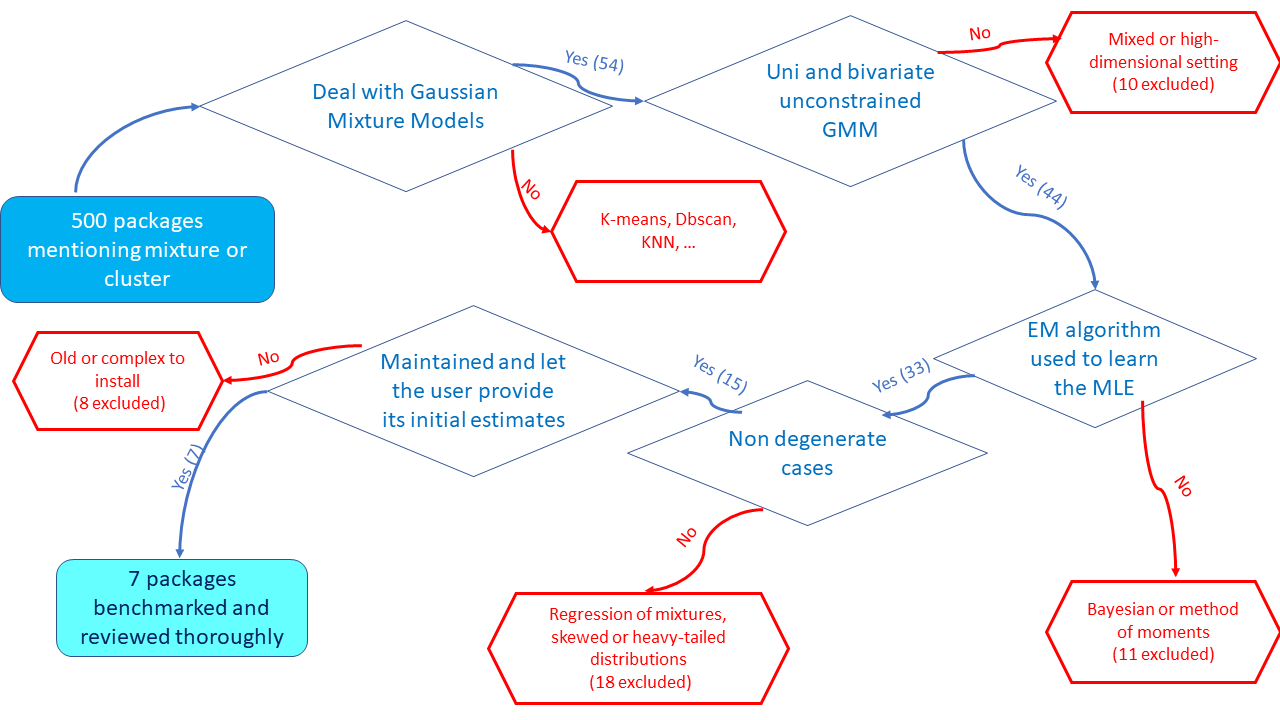
\includegraphics[width=1\linewidth]{figures/flowchart_packages_selection} 

}

\caption{A minimal roadmap used for the selection of the packages reviewed in our benchmark.}\label{fig:flowchart}
\end{figure}

We also include two additional packages dedicated specifically to high-dimensional settings, namely \CRANpkg{EMMIXmfa} (Rathnayake et al. 2019) and \CRANpkg{HDclassif} (Berge, Bouveyron, and Girard 2019) to compare their performance with standard multivariate approaches in complex, but non degenerate cases. We summarise the main features and use cases of the seven + two reviewed
packages in Table
\ref{tab:low-comparison-package-pdf}.
The three most commonly used packages are \pkg{mixtools}, \pkg{mclust} and \pkg{flexmix}. However, the \pkg{mclust} package is by far the most complete with many features provided to visualise and evaluate the quality of the GMM estimate. \pkg{bgmm} has the greatest number of dependencies, while \pkg{mclust} only depends of base R packages. Additionally, in parallel to clustering tasks, \pkg{flexmix} and \pkg{mixtools} packages perform
regression of mixtures and implement mixture models using other
parametric distributions or non-parametric methods via kernel-density
estimation.

\begin{table}[!h]

\caption{\label{tab:low-comparison-package-pdf}Main features of the reviewed packages, sorted by decreasing number of daily downloads.
               \textit{Downloads per day} returns the daily average number of downloads for each package on the last 2 years.
               \textit{Recursive dependencies} column counts the complete set of non-base packages required,
               as first-order dependencies depend on other packages as well.}
\centering
\resizebox{\linewidth}{!}{
\begin{tabular}[t]{llllrllrl}
\toprule
\multicolumn{1}{c}{\textbf{Package}} & \multicolumn{1}{c}{\textbf{Version}} & \multicolumn{1}{c}{\textbf{Regression}} & \multicolumn{1}{c}{\textbf{\makecell[l]{Implemented \\ models}}} & \multicolumn{1}{c}{\textbf{\makecell[c]{Downloads \\ per day}}} & \multicolumn{1}{c}{\textbf{\makecell[r]{Last \\ update}}} & \multicolumn{1}{c}{\textbf{Imports}} & \multicolumn{1}{c}{\textbf{\makecell[c]{Recursive \\ dependencies}}} & \multicolumn{1}{c}{\textbf{Language}}\\
\midrule
\midrule
mclust & 5.4.7 & $
\includegraphics[scale=0.05]{figures/red_cross.png}$ & $
\includegraphics[scale=0.05]{figures/red_cross.png}$ & 5223 & 31/10/2022 & R ($\ge$ 3.0) & 0 & Fortran\\
flexmix & 2.3-17 & 
\includegraphics[scale=0.05]{figures/green_tick.png}& \makecell[c]{Poisson, binary,\\non-parametric,\\semi-parametric} & 3852 & 07/06/2022 & \makecell[c]{R ($\ge$ 2.15.0), modeltools,\\nnet, stats4} & 3 & R\\
mixtools & 1.2.0 & 
\includegraphics[scale=0.05]{figures/green_tick.png}& \makecell[r]{multinomial, gamma,\\Weibull, non-parametric,\\semi-parametric} & 178 & 05/02/2022 & \makecell[r]{R ($\ge$ 3.5.0), kernlab,\\segmented, survival} & 6 & C\\
Rmixmod & 2.1.5 & $
\includegraphics[scale=0.05]{figures/red_cross.png}$ & $
\includegraphics[scale=0.05]{figures/red_cross.png}$ & 39 & 18/10/2022 & \makecell[l]{R ($\ge$ 2.12.0), Rcpp,\\RcppEigen} & 4 & C++\\
EMCluster & 0.2-13 & $
\includegraphics[scale=0.05]{figures/red_cross.png}$ & $
\includegraphics[scale=0.05]{figures/red_cross.png}$ & 33 & 12/08/2022 & R ($\ge$ 3.0.1), Matrix & 3 & C\\
\addlinespace
bgmm & 1.8.4 & $
\includegraphics[scale=0.05]{figures/red_cross.png}$ & $
\includegraphics[scale=0.05]{figures/red_cross.png}$ & 27 & 10/10/2021 & \makecell[r]{\\R ($\ge$ 2.0),\\mvtnorm, combinat} & 77 & R\\
GMKMcharlie & 1.1.1 & $
\includegraphics[scale=0.05]{figures/red_cross.png}$ & $
\includegraphics[scale=0.05]{figures/red_cross.png}$ & 12 & 29/05/2021 & \makecell[l]{Rcpp, RcppParallel,\\RcppArmadillo} & 3 & C++\\
\midrule
EMMIXmfa & 2.0.11 & $
\includegraphics[scale=0.05]{figures/red_cross.png}$ & $
\includegraphics[scale=0.05]{figures/red_cross.png}$ & 12 & 16/12/2019 & NA & 0 & C\\
HDclassif & 2.2.0 & $
\includegraphics[scale=0.05]{figures/red_cross.png}$ & $
\includegraphics[scale=0.05]{figures/red_cross.png}$ & 35 & 12/10/2022 & rARPACK & 13 & R\\
\bottomrule
\end{tabular}}
\end{table}

We further detail features specifically related to GMMs in Table
\ref{tab:high-comparison-packages-pdf}. We detail row after row its content below:

\begin{itemize}
\item
  The parametrisations used to provide parsimonious estimation of the GMMs are reviewed in \protect\hyperlink{parameter-estimation-in-finite-mixtures-models}{Parameter estimation in finite mixtures models} and summarised in rows 1 and 2 (Table \ref{tab:high-comparison-packages-pdf}) for the univariate and multivariate setting. We refer to the package as ``canonical'' when it implements both homoscedastic and heteroscedastic parametrisations in the univariate setting, and the 14 parametrisations listed in Supplementary Table 3 in the multivariate setting. Adding the additional constraint of equi-balanced clusters results in a total to \(14 \times 2=28\) distinct models and \(2 \times 2=4\) parametrisations, respectively in the univariate and multivariate setting. Since \pkg{EMMIXmfa} and \pkg{HDclassif} are dedicated to the analysis of high-dimensional datasets, they project the observations in a smaller subspace and are not available in the univariate setting. Given an user-defined or prior computed intrinsic dimension, we can imagine using any of the standard parametrisations available for instance in the \pkg{mclust} package, and listed in Appendix \emph{Parsimonious parametrisation of multivariate GMMs}. In addition, \pkg{HDclassif} allows each cluster \(j\) to be represented with its own subspace intrinsic dimension \(d_j\), as we describe in further details in Appendix \emph{Parameters estimation in a high-dimensional context}.
\item
  \protect\hyperlink{the-em-algorithm}{The EM algorithm} is the most commonly employed method for estimating the parameters of GMMs, however, alternative algorithms based on the EM framework, are reviewed in Appendix B: \emph{Extensions of the EM algorithm to overcome its limitations} and row 3 of Table \ref{tab:high-comparison-packages-pdf}. Especially, GMMs estimation is particularly impacted by the presence of outliers, justifying a specific benchmark (see Appendix \emph{A small simulation to evaluate the impact of outliers}).
  We briefly review the most common initialisation algorithms in section \protect\hyperlink{initialisation-of-the-em-algorithm}{Initialisation of the EM algorithm} and row 4 of Table \ref{tab:high-comparison-packages-pdf}, a necessary and tedious task for both the EM algorithm and its alternatives.
\item
  To select the best parametrisations and number of components that fit the mixture, several metrics are provided by the reviewed packages (\emph{Model selection} and row 5). Due to the complexity of computing the true distribution of the estimated parameters, bootstrap methods are commonly used used to derive confidence intervals (see Appendix \emph{Derivation of confidence intervals in GMMs} and row 6 in Table \ref{tab:high-comparison-packages-pdf}).
\end{itemize}

\begin{itemize}
\tightlist
\item
  Six packages supply several functions for visualisation, summarised in the last row of Table \ref{tab:high-comparison-packages-pdf}, to display either the distributions corresponding to the estimated parameters or compare quickly the performance across packages. However, \pkg{mclust} is by far the most complete one, with density plots (in the univariate setting) and isodensity plots (bi-dimensional in the bivariate setting or in higher dimensions after appropriate dimensionality reduction), with the option to plot custom confidence intervals and critical regions, and finally boxplot bootstrap representations for displaying the distribution of the benchmarked estimated parameters.
\end{itemize}

High-dimensional packages provide specific representations adjusted to the high-dimensional settings, notably allowing the user to visualise the projected factorial representation of its dataset in a two or three-dimensional subspace. They also provide specialised performance plots, notably scree plots or BIC scatter plots to represent in a compact way numerous projections and parametrisations.

\begin{table}[!h]

\caption{\label{tab:high-comparison-packages-pdf}Custom features associated to GMMs estimation for any of the benchmarked packages.}
\centering
\resizebox{\linewidth}{!}{
\begin{tabular}[t]{>{}l|>{\raggedright\arraybackslash}m{4cm}>{\raggedright\arraybackslash}m{1.6cm}>{\raggedright\arraybackslash}m{1.6cm}>{\raggedright\arraybackslash}m{1.6cm}>{\raggedright\arraybackslash}m{1.6cm}>{\raggedright\arraybackslash}m{1.6cm}>{}l|>{\raggedright\arraybackslash}m{1.6cm}>{\raggedright\arraybackslash}m{1.6cm}}
\toprule
\multicolumn{1}{c}{\textbf{ }} & \multicolumn{1}{c}{\textbf{mclust}} & \multicolumn{1}{c}{\textbf{flexmix}} & \multicolumn{1}{c}{\textbf{mixtools}} & \multicolumn{1}{c}{\textbf{Rmixmod}} & \multicolumn{1}{c}{\textbf{EMCluster}} & \multicolumn{1}{c}{\textbf{bgmm}} & \multicolumn{1}{c}{\textbf{GMKMcharlie}} & \multicolumn{1}{c}{\textbf{EMMIXmfa}} & \multicolumn{1}{c}{\textbf{HDclassif}}\\
\midrule
\textbf{Models Available (univariate)} & canonical & unconstrained & canonical & canonical & unconstrained & canonical & unconstrained & NA & NA\\
\midrule
\textbf{Models Available (multivariate)} & canonical & unconstrained diagonal or general & unconstrained & canonical & unconstrained & 4 models (diagonal and general, either component specific or global) & unconstrained & 4 models (either component-wise or common, on the intrinsic and diagonal residual error covariance matrices) & canonical on projected dimension\\
\midrule
\textbf{Variants of the EM algorithm} & VBEM & SEM, CEM & ECM & SEM, CEM & 
\includegraphics[scale=0.05]{figures/red_cross.png}& 
\includegraphics[scale=0.05]{figures/red_cross.png}& CW-EM, MML & AECM & SEM, CEM\\
\midrule
\textbf{Initialisation} & hierarchical clustering, quantile & short-EM, random & random & random, short-EM, CEM, SEM & random, short-EM & k-means, quantile & k-means & k-means, random, heuristic & short-EM, random, k-means\\
\midrule
\textbf{Model or Cluster Selection} & BIC, ICL, LRTS & AIC, BIC, ICL & AIC, BIC, ICL, CAIC, LRTS & BIC, ICL, NEC & AIC, BIC, ICL, CLC & GIC & 
\includegraphics[scale=0.05]{figures/red_cross.png}& 
\includegraphics[scale=0.05]{figures/red_cross.png}& BIC, ICL, CV\\
\midrule
\addlinespace
\textbf{Bootstrap Confidence Intervals} & 
\includegraphics[scale=0.05]{figures/green_tick.png}& 
\includegraphics[scale=0.05]{figures/green_tick.png}& 
\includegraphics[scale=0.05]{figures/green_tick.png}& 
\includegraphics[scale=0.05]{figures/red_cross.png}& 
\includegraphics[scale=0.05]{figures/red_cross.png}& 
\includegraphics[scale=0.05]{figures/red_cross.png}& 
\includegraphics[scale=0.05]{figures/red_cross.png}& 
\includegraphics[scale=0.05]{figures/red_cross.png}& 
\includegraphics[scale=0.05]{figures/red_cross.png}\\
\midrule
\textbf{Visualisation} & performance, histograms and boxplots of bootstrapped estimates, density plots (univariate),  scatter plots with uncertainity regions and boundaries (bivariate), isodensity (bivariate , 2D projected PCA or selecting coordinates) & 
\includegraphics[scale=0.05]{figures/red_cross.png}& density curves & density curves, scatter plots with uncertainty boundaries & 
\includegraphics[scale=0.05]{figures/red_cross.png}& performance, scatter plots with uncertainty boundaries & 
\includegraphics[scale=0.05]{figures/red_cross.png}& projected factorial map & projected factorial map, performance (Cattell's scree plot, BIC performance, slope heuristic)\\
\midrule
\bottomrule
\end{tabular}}
\end{table}

\hypertarget{methods}{%
\subsection{Methods}\label{methods}}

In addition to the the seven packages selected for our benchmark, we
include a custom R implementation of the EM algorithm used
as baseline, referred to as \emph{RGMMBench}, and for the high-dimensional setting we select packages \pkg{EMMIXmfa} and \pkg{HDclassif}, on the basis of criteria detailed in Appendix C, \emph{General workflow}. Code for \emph{RGMMBench} is provided in Appendix \emph{Application of the EM algorithm to GMMs}. To compare the statistical performances of these packages, we performed \emph{parametric bootstrap} (\emph{Derivation of confidence intervals in GMMs}) and built an experimental design to cover distinct mixture distributions parameter configurations, using prior user-defined parameters.

For each experiment, we assign each observation to an unique cluster by drawing \(n\) labels \(S_{1:n}\) from a multinomial distribution whose parameters were the prior user-defined proportions \(p=(p_1, \ldots, p_k)\). Then, each observation \(x_i\) assigned to hidden component \(j\) is drawn from a Normal distribution using the \code{stats::rnorm()} function for the univariate distribution and \code{MASS::mvrnorm} for the multivariate distribution. The complete code used for simulating data is
available on GitHub at \href{https://github.com/bastienchassagnol-servier/RGMMBench}{RGMMBench}. Finally, we obtain an empirical distribution of the estimated parameters by computing the MLE
of each randomly generated sample.

For all the packages, we used the same convergence threshold, \(10^{-6}\), and maximum of 1,000 iterations, as a numerical criterion for convergence. We generated simulated data with \(n = 200\) observations in the univariate setting and \(n = 500\) observations in the bivariate setting. We set the number of observations in order to minimise the probability of generating a sample without drawing any observations from one of the components\footnote{It is especially critical in cases of highly unbalanced configurations, as detailed in Appendix \emph{Practical details for the implementation of our benchmark}}. Unless stated explicitly, we kept the default hyper-parameters and custom global options provided by each package. For instance, the \pkg{flexmix} package has a default option, \emph{minprior}, set by default to 0.05, which removes any component present in the mixture with a ratio below \(0.05\). Besides, the fully unconstrained model was the only one which we implemented both in the univariate and multivariate settings, as it is the only parametrisation implemented in all the seven packages.

We compared the packages' performances using five
initialisation methods: random, quantile, \emph{k}-means, rebmix and hierarchical clustering in the univariate setting. We benchmarked the same initialisation methods in the multivariate setting, except for the quantile method which has no multivariate equivalent (see section \protect\hyperlink{initialisation-of-the-em-algorithm}{Initialisation of the EM algorithm}):

\begin{itemize}
\item
  We used the function \code{EMCluster::rand.EM()} with 10 random restarts and minimal cluster size of 2 for the random initialisation. The method implemented by \pkg{EMCluster} is the most commonly used, described in details in Biernacki, Celeux, and Govaert (2003) and in section \protect\hyperlink{initialisation-of-the-em-algorithm}{Initialisation of the EM algorithm}.
\item
  To implement the k-means initialisation, we used the \code{stats::kmeans()} function with a convergence criterion fo 10\^{}\{-2\} and maximum of 200 iterations. The initial centroid and covariance matrix for each component were computed by restricting to the sample observations assigned to the corresponding component. The approach is close to the one adopted by the CEM algorithm (see Appendix B: \emph{Extensions of the EM algorithm to overcome its limitations}).
\item
  We used the \code{mclust::hcV()} function for the MBHC algorithm. This method has two main limitations: just like the \emph{k}-means implementation, it only returns a cluster assignment to each observation instead of the posterior probabilities, and the splitting process to generate the clusters sometimes results in clusters composed of only one observation. To avoid this, we added a small epsilon to each posterior probability.
\item
  We used in the univariate setting \code{bgmm::init.model.params} for the quantiles initialisation.
\item
  To implement the rebmix method, we used the \code{rebmix::REBMIX} function, using the \emph{kernel density estimation} for the estimation of the empirical density distribution coupled with \emph{EMcontrol} set to one to prevent the algorithm from starting EM iterations.
\item
  Any of the seven packages could be used to implement the small EM method. We decided to use the \code{mixtools::normalmixEM} as it is the closest one to our custom implementation. We specified 10 random restarts, a maximal number of iterations of 200 and an alleviated absolute threshold of \(10^{-2}\). Preliminary experiments have led us to consider the removal of the small EM initialization method from the simulation benchmark. This decision is based on the observation that the differences of performance observed between the packages were no longer significant (see supplementary Figure 9).
\end{itemize}

We sum up in Table \ref{tab:general-parameter-description-pdf} the general configuration used to run the scripts. Additionally, all simulations were run with the same R (R Core Team 2023) version 4.0.2 (2020-06-22).

\begin{table}[!h]

\caption{\label{tab:general-parameter-description-pdf}Global options shared by all the benchmarked packages.}
\centering
\resizebox{\linewidth}{!}{
\begin{tabular}[t]{>{\centering\arraybackslash}p{4.1cm}>{\centering\arraybackslash}p{4.1cm}>{\centering\arraybackslash}p{4.1cm}>{\centering\arraybackslash}p{4.1cm}>{\centering\arraybackslash}p{4.1cm}}
\toprule
Initialisation methods & Algorithms & Criterion threshold & Maximal iterations & Number of observations\\
\midrule
midrule
hc, kmeans, small EM,rebmix, quantiles, random & EM R, Rmixmod, bgmm, mclust, flexmix, EMCluster, mixtools, GMKMCharlie & $10^{-6}$ & 1000 & 100, 200, 500, 1000, 2000, 5000, 10000\\
\bottomrule
\end{tabular}}
\end{table}

Preliminary experiments suggested that the quality of the estimation of a GMM is mostly affected by the overlap between components' distribution and level of unbalance between components. We quantified the overlap between two components by the following overlap score (OVL, see Equation \eqref{eq:overlap}), with a smaller score denoting well-separated components:

\begin{equation}
       \operatorname{OVL}(i, j) = \int \min (f_{\zeta_i} (x), f_{\zeta_j} (x)) dx \quad \text{ with } i \neq j
  \label{eq:overlap}
\end{equation}

We may generalise this definition to \(k\) components by averaging the
individual components' overlap. We use the function
\code{MixSim::overlap} from the \CRANpkg{MixSim} package (Melnykov, Chen, and Maitra 2021) that approximates this quantity using a Monte-Carlo based method (see appendices \emph{An analytic formula of the overlap for univariate Gaussian mixtures} and \emph{Practical details for the implementation of our benchmark} for further details).

The level of imbalance may be evaluated with entropy measure (Equation \eqref{eq:entropy}):

\begin{equation}
    H(S)=-\sum_{j=1}^k p_j \log_k (p_j)
\label{eq:entropy}
\end{equation}

with \(k\) is the number of components and \(p_j=\mathbb{P}(S=j)\) is the frequency of class \(j\).

We considered 9 distinct configuration parameters, associated with distinct values of \(\operatorname{OVL}\) and entropy in the univariate setting, 20 configurations in the bivariate setting, and 16 configurations in the high-dimensional setting. Briefly, in the univariate setting, we simulated components with the same set of four means (0, 4, 8, and 12), three sets of mixture proportions\\
\(\left[(0.25, 0.25, 0.25, 0.25); (0.2, 0.4, 0.2, 0.2); (0.1, 0.7, 0.1, 0.1) \right]\) and three variances: \((0.3, 1, 2)\). In the bivariate setting, we consider two sets of proportions: \(\left[(0.5, 0.5); (0.9, 0.1) \right]\), two sets of coordinate centroids: \(\left[(0; 20), (20, 0) \right]\) and \(\left[(0; 2), (2, 0) \right]\), the same variance of 1 for each feature and for each component for illustrative purposes of the direct relation linking the correlation and the level of OVL and five sets of correlation:\([(-0.8, -0.8); (0.8, -0.8); (-0.8, 0.8); (0.8, 0.8); (0, 0)]\).

Finally, we tested eight configurations in the high-dimensional framework, setting to \(D=10\) the number of dimensions. We modified the level of overlap (definition is reported in Equation \eqref{eq:overlap}) and the imbalance between the component proportions across our simulations. Additionally, we tested two types of constraints on the covariance matrix: fully parametrised and spherical (see Appendix \emph{Parsimonious parametrisation of multivariate GMMs}). Each of the parameter configurations tested in the high-dimensional setting was evaluated with \(n=200\) observations and \(n=2000\) observations. Additionally, instead of manually defining the parameters for the high-dimensional simulation, we used the \code{MixSim} function from the \CRANpkg{MixSim} package (Melnykov, Chen, and Maitra 2021). This function returns the user a fully parametrised GMM, with a prior defined level of maximum or average overlap\footnote{Unfortunately, as discussed in further details in Appendix \emph{An analytic formula of the overlap for univariate Gaussian mixtures}, the MixSim package does not compute the global distribution overlap, but instead returns the mean of pairwise overlap between any component (however, with two components, these two alternative definitions match.) Finally, it is not possible to set the proportions of the components before the generation of the parameters, except for clusters with equal proportions, and contrary to the expect behaviour of additional parameter \emph{PiLow}, supposed to define the smallest mixing proportion.}.

The complete list of parameters used is reported respectively in Table \ref{tab:parameter-configuration-univariate} for the univariate setting, Table \ref{tab:parameter-configuration-bivariate} for the bivariate setting and \ref{tab:parameter-configuration-HD} for the high-dimensional setting. We benchmarked simulations where the components were alternatively very distinct or instead very overlapping, as well as of equal proportions or instead very unbalanced. The adjustments made to meet the specific requirements of high dimensional packages are detailed in \emph{Practical details for the implementation of our benchmark}.

We report the most significant results and features and the associated recommendations in next section \protect\hyperlink{results}{Results}.

\hypertarget{results}{%
\subsection{Results}\label{results}}

All figures and performance overview tables are reported in \emph{Supplementary Figures and Tables in the univariate simulation} for the univariate setting, \emph{Supplementary Figures and Tables in the bivariate simulation} for the bivariate scenario and \emph{Supplementary Figures and Tables in the HD simulation} for the high dimensional scenario.

\textbf{Balanced and non-overlapping components}

In the univariate setting, with balanced components and low \(\operatorname{OVL}\) (scenario U1 in Table
\ref{tab:parameter-configuration-univariate}), the parameter
estimates are identical in most cases across initialisation methods and packages, notably the same estimates are returned with \emph{k}-means or rebmix initialisation. However, the random initialisation method leads
to a higher variance and bias on the parameter estimates than other
methods (Supplementary Figure 4 and Supplementary Table 6),
with some estimates fitting only local maxima, far from the optimal value.

Similarly, the scenarios in the bivariate setting (configurations B6-B10 in Table \ref{tab:parameter-configuration-bivariate}), with a focus on B6, B7 and B10 visualised in Supplementary Figure 16, feature well-separated and balanced components. Consistent with conclusions from the corresponding univariate configurations, all benchmarked packages return the same estimates across initialisation methods.

\textbf{Unbalanced and non-overlapping components}

However, with unbalanced classes and low \(\operatorname{OVL}\) (scenario U7 in
\ref{tab:parameter-configuration-univariate}), the choice of the
initialisation method is crucial, with quantiles and random
methods yielding more biased estimates and proned to fall in local maximum. Rebmix initialisation provides the best estimates, with the smallest MSE and bias across packages (Supplementary Figure
5 and supplementary Table 7, always associated with the highest likelihood. Overall, with
well-discriminated components, most of the differences on the estimation
originate from the choice of initialisation method, while the choice of
the package has only small impact.

In the bivariate framework, two configurations featured both strongly unbalanced and well-separated components, similarly to scenario U3 in Table \ref{tab:parameter-configuration-univariate}: the configurations B12 (Supplementary Figure 12 and Table 12) and B14 (Supplementary Figure 13 and Supplementary Table 13). Similarly, configurations B16, B17 and B20 (Table \ref{tab:parameter-configuration-bivariate}) with similar characteristics are summarised in supplementary Figure 17. In all these configurations, neither the initialisation method nor the package have a statistical significant impact on the overall performance.

Similarly, configurations HD1a-HD4b in Table \ref{tab:parameter-configuration-HD}) in the high dimensional setting display well-separated clusters, with a representative outcome represented in Supplementary Figure 19 and Supplementary Table 16. Consistent with the results obtained in the analogous univariate and bivariate scenarios, in the unbalanced and non-overlapping framework, the majority of the benchmarked packages produce highly consistent and similar estimates when hierarchical clustering and k-means were used for parameter initialisation. However, \pkg{bgmm} and \pkg{EMCluster} clearly perform worse when the rebmix initialization method is used (however, overall, rebmix performs poorly, regardless of the package used for estimation). Notably, initialisations with the rebmix package tend to display a much larger number of poor estimations, some of which can be identified with the local maxima associated with parameter switching between the two classes. Finally, the two additional packages dedicated to high-dimensional clustering display the worst performances, with \pkg{EMMIXmfa} returning the most biased parameters and \pkg{HDclassif} the most noisy estimates. \pkg{EMMIXmfa} is the only package that returned highly biased estimates of the components' proportions in this setting.

\textbf{Balanced and overlapping components}

When the overlap between components increases, the bias and variability of the estimates tends to increase, and the choice of initialisation method becomes more impactful.
The least biased and noisy estimations with balanced components in the univariate setting (scenario U3 in Table
\ref{tab:parameter-configuration-univariate}) are obtained with
the \emph{k}-means initialisation (Supplementary Figure
3 and Table 8) while the rebmix initialisation returns the most biased and noisy
estimates. Similar results are found in the bivariate setting with a balanced and highly overlapping two-component GMM (configurations B1-B5 from Table \ref{tab:parameter-configuration-bivariate}), with the best performance reached with the \emph{k}-means initialisation method, followed by MBHC. This is emphasised in supplementary Figure 16, in the top three most complex configurations, namely B1, B2 and B5. If the shape of the covariance matrix is well-recovered, no matter the package, the Hellinger distances are significantly higher (and thus the estimate further away from the target distribution) with the random and rebmix methods.

Similarly, in the high-dimensional scenario HD7 of Table \ref{tab:parameter-configuration-HD}), presenting balanced but highly overlapping clusters with a full covariance structure, the best performance was obtained with \emph{k}-means initialisation, while the rebmix initialisation returned the most biased and noisy estimates. While \pkg{EMMIXmfa} performed well when it converged, it returned an error in most cases (see Column \emph{Success} of supplementary Table 17). The least biased estimates were returned by \pkg{mixtools} and \pkg{Rmixmod} and the least noisy by \pkg{flexmix}, \pkg{mclust} and \pkg{GMKMCharlie} (smaller MSE). Interestingly, in the high-dimensional setting, the packages \pkg{EMCluster} and \pkg{bgmm} exhibited worse performance. In particular, as can be seen in panel E of supplementary Figure 20, the proportions of the components recovered the \(]0-1[^k\) simplex.

Conversely, the \pkg{EMCluster} package, and to a lesser extent, the \pkg{bgmm} package, performed surprisingly well when datasets were simulated with an underlying spherical covariance structure, even though the estimation was not performed explicitly with this constraint (Supplementary Table 19). Indeed, it seems like that the off-diagonal terms tended to converge towards 0, as showcased in Supplementary Figure 21, in Panel C, in which the fourth row from top represents the bootstrap intervals associated to the pairwise covariance between dimension 1 and 2 of each cluster.

\textbf{Unbalanced and overlapping components}

With unbalanced components and high \(\operatorname{OVL}\) (scenario U9 in Table
\ref{tab:parameter-configuration-univariate}), all packages, no
matter the initialisation method, provided biased estimates, with a higher variability of the parameter estimates compared to other configurations. The least biased
estimates were obtained with \emph{k}-means or random initialisation, but with a higher variability on the estimates with random initialisation (Supplementary Table 9).
Delving further into the individual analysis of the parameter estimates associated to each component, we found out that the least biased estimates were achieved with rebmix initialisation for the most distinguishable components. For instance, in our configuration, the clusters 2 and 4 (see Supplementary Figure 7 and Table 9) were better characterised with the rebmix method. This observation aligns with the rebmix's underlying framework, using the modes of the distribution for initialising the component (Nagode 2015). With highly-overlapping distributions and unbalanced components, both the choice of the initialisation algorithm and the package have a
substantial impact on the quality of the estimation of this mixture.

Two configurations in our bivariate simulation feature distributions with both strong OVL and unbalanced components. Especially, the scenario B11 (Table \ref{tab:parameter-configuration-bivariate}) has the strongest OVL overall, with notably a risk of wrongly assigning minor component 2 to major component 1 of 0.5 (a random method classifying each observation to cluster 1 or 2 would have the same performance).

First, we observe that the the random and rebmix initialisation methods have similar performance, significantly better than \(k\)-means or MBHC (Supplementary Figure 11). Specifically, the rebmix method returns the least biased estimates, while the random method is associated with the lowest MSE (respectively for configurations B11 and B15, the supplementary Tables 11
and 14). Second, the estimates differ across packages only in these two complex configurations, with packages \pkg{Rmixmod} and \pkg{mixtools} returning more accurate estimates than the others.
It it is particularly emphasised in Scenario B15, where the component-specific covariance matrices are diagonal with same non-null input, and thus should present spherical density distributions. However, only the first class of packages correctly recovers the spherical bivariate \(95\%\) confidence regions while they are slightly ellipsoidal with the second class of packages (Panel B, Supplementary Figure 14).

With full covariance structures and unbalanced proportions, as depicted in the high-dimensional Scenario HD8a) and b) of Table \ref{tab:parameter-configuration-HD}, the general observations stated in the previous subsection for the high dimensional setting hold, namely that the least biased estimates are returned by packages not specifically designed for high-dimensional data, with the \emph{k}-means initialisation (Supplementary Table 12 and supplementary Figure 22). Furthermore, the \pkg{EMCluster} and \pkg{bgmm} packages and the two packages dedicated to high-dimensional, perform similarly with \(n=200\) observations (sub-scenario a) and \(n=2000\) observations (sub-scenario b), whereas we would expect narrower and less biased confidence intervals by increasing the number of observations by a factor of 10.

Finally, with spherical covariance structures and unbalanced proportions, the best performances, both in terms of bias and variability, are obtained with \pkg{flexmix}, \pkg{mclust} and \pkg{GMKMCharlie}. Indeed, as detailed later in \protect\hyperlink{conclusions}{Conclusions}, these packages are more sensitive to the choice of the initialisation method and have a greater tendency to get trapped in the neighbourhood of the initial estimates (Supplementary Table 19 and supplementary Figure 22). Accordingly, \emph{k}-means initialisation performs best since it assumes independent and homoscedastic features for each cluster.
Furthermore, \pkg{EMMIXmfa} is the package that best estimates the off-diagonal terms in this setting, as highlighted in supplementary Table 19.

\textbf{Identification of two classes of packages with distinct behaviours}

By summarizing the results obtained across all simulations, we identify two classes of packages with distinct behaviours (Figure
\ref{fig:dichotomy-package-conclusion}):

\begin{itemize}
\item
  The first class of packages, represented by \pkg{Rmixmod} and \pkg{mixtools}, returns similar estimates to our baseline EM implementation. The estimates returned by these packages are less biased but at the extent of a higher variability on the estimates. Additionally, with overlapping mixtures, they tend to be slower compared to the second class, since they require additional steps to reach convergence.
\item
  The second class of packages, composed of the other
  reviewed packages, is more sensitive to the initialisation method. This leads to more
  biased but less variable estimates, especially when assumptions done by
  the initialisation algorithm are not met.
\end{itemize}

Panels A, B and C display, respectively in the univariate, bivariate and high-dimensional setting, the heatmap of the Pearson correlation between the estimated parameters across the benchmarked packages for the most discriminative scenario (the one featuring the most unbalanced and overlapping components): scenario U9, Table \ref{tab:parameter-configuration-univariate} in the univariate setting, scenario B11, Table \ref{tab:parameter-configuration-bivariate}, for the bivariate simulation and scenario HD8, Table \ref{tab:parameter-configuration-HD} for the high-dimensional simulation, with the \emph{k}-means initialisation.

We further identified with this representation minor differences for the estimation of the parameters between \pkg{Rmixmod} and \pkg{mixtools}, while three subgroups can be identified in the second class of packages: the first subset with \pkg{bgmm} and \pkg{mclust}, the second subset with \pkg{EMCluster} and \pkg{GMKMcharlie} packages and the \pkg{flexmix} package, which clearly stands out from the others, as being the one most likely to be trapped at the boundaries of the parameter space. After examining the source codes of the packages, we attribute this differences to custom implementation choices of the EM algorithm, such as the way numerical underflow is managed or the choice of a relative or absolute scale to compare consecutive computed log-likelihoods (see Appendix \emph{EM-implementation differences across reviewed packages} and Panel D, Figure \ref{fig:dichotomy-package-conclusion}). In the high-dimensional setting, the second class of packages showed additional heterogeneity, with \pkg{EMCluster} and \pkg{bgmm} setting themselves apart from the other three packages.

\begin{figure}

{\centering 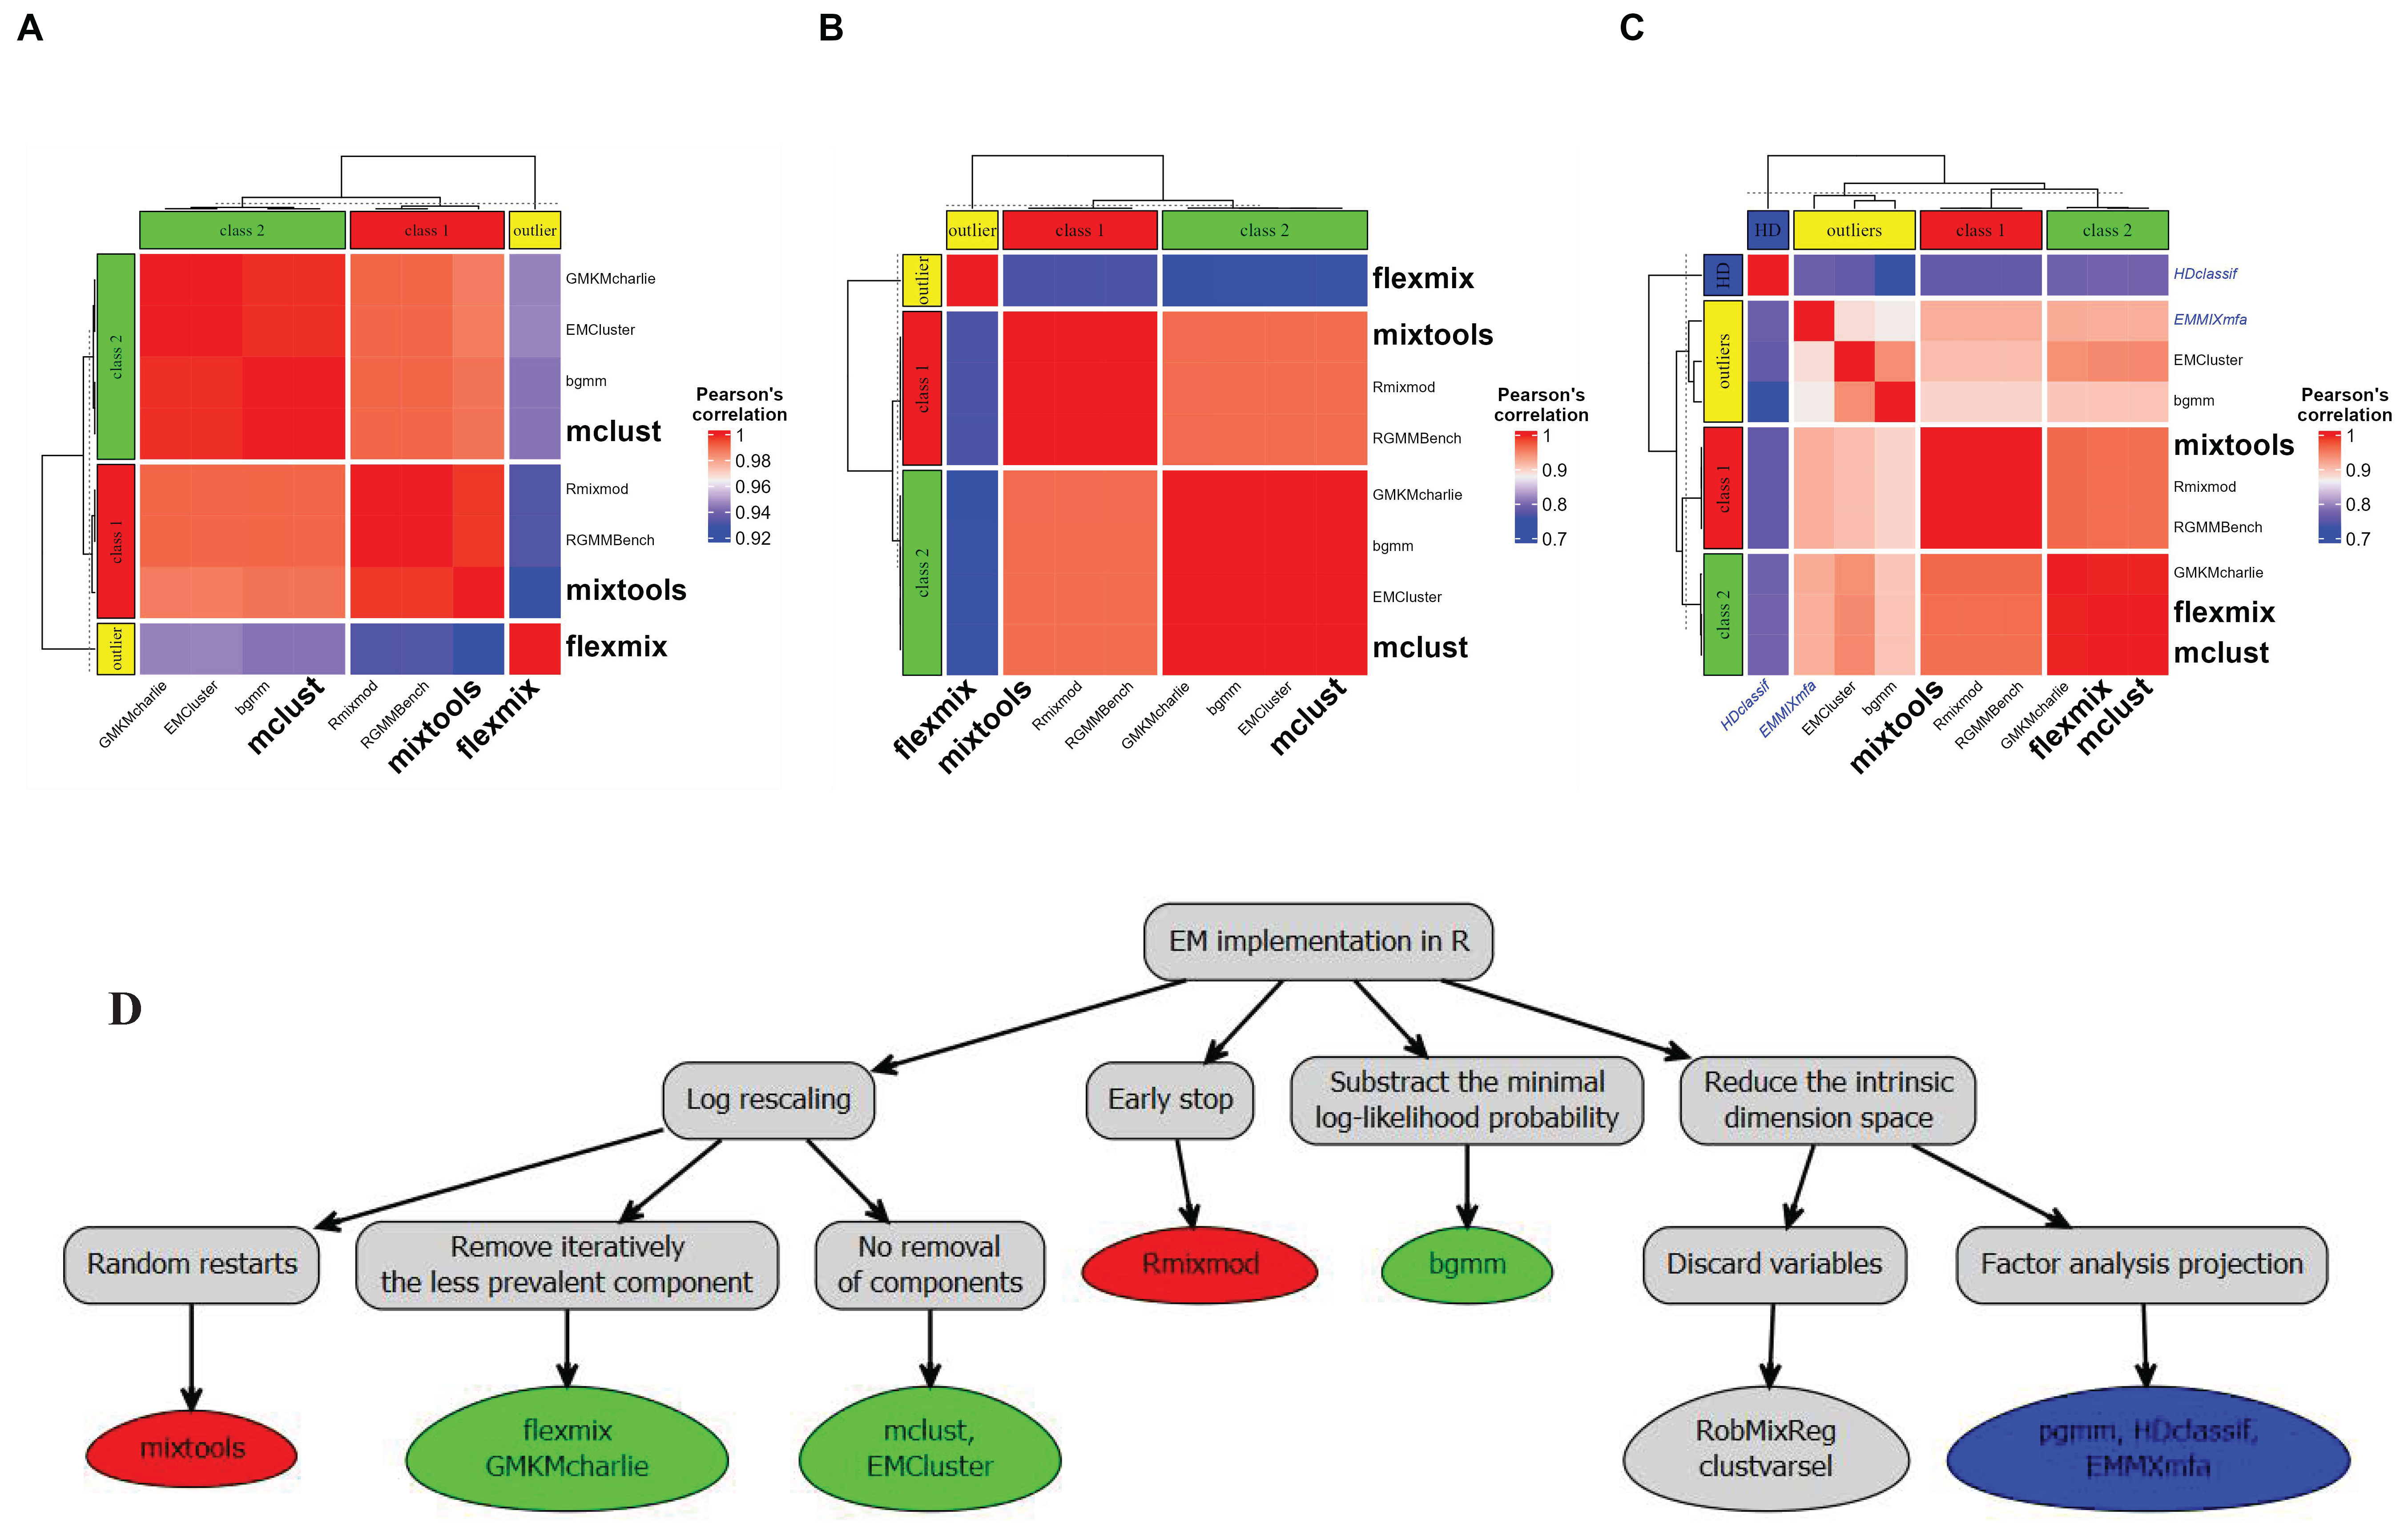
\includegraphics[width=1\linewidth]{./figures/dichotomy_package_conclusion} 

}

\caption{Panels A, B and C show respectively the heatmap of the Pearson correlation in the univariate, bivariate and high-dimensional framework between the parameters estimated by the packages, evaluated for the most discriminating and complex scenario. The correlation matrix was computed using the function \code{stats::cor} with option \textit{complete} to remove any missing value related to a failed simulation, and the heatmap generated with the Bioconductor package \BIOpkg{ComplexHeatmap}. Panel D represents a tree summarising the main differences between the benchmarked packages, in terms of the EM implementation. They are discussed in more detail in Appendix \textit{EM-implementation differences across reviewed packages}.}\label{fig:dichotomy-package-conclusion}
\end{figure}

\textbf{Failed estimations}

Finally, in some cases, neither the specific EM algorithm implemented by each package nor the initialisation method were able to return an estimate with the expected number of components, or converged to a degenerate distribution (e.g., with infinite or zero variances). In that case, we considered the estimation as failed and accordingly we did not include it into the visualisations and the summary metric tables.

Most of the failed estimations occurred with the rebmix initialisation. Indeed, an updated version of the package forced the user to provide a set of possible positive integer values for the number of components, with at least a difference of two between the model with the most components and the model with the least components (we therefore set the parameter \emph{cmax} to \(k+1\) and \emph{cmin} to \(k-1\)).In scenarios where the distributions associated with each cluster exhibit significant overlap, there is an increased risk of incorrectly estimating the number of components. This arises from the inherent difficulty of discerning the modes within the overall distribution. For instance, in the most complex scenario B11, characterized by strong overlap and imbalanced clusters (refer to Table \ref{tab:parameter-configuration-bivariate}), up to \(20\%\) of initialisations were unsuccessful. Similarly, in the second most challenging scenario, B15, approximately \(10\%\) of initializations failed against an averaged number of \(4\%\) of the simulations exhibiting an inaccurate estimation of the number of components.

Removing errors proceeding from the initialisation method, only the \pkg{flexmix} package failed in returning an estimate matching the user criteria in some configurations of the univariate and bivariate settings. In both cases, the strong assumption that any cluster with less than \(5\%\) of the observations is irrelevant, results in trimming one or more components\footnote{With a two-components mixture like our bivariate scenario, this even implies to consider an unimodal distribution of the dataset}. This strong agnostic constraint on component proportions led to failures in configurations featuring strongly overlapping clusters, with up to \(20\%\) failed estimations with the random initialisation method in scenario B11 (Table \ref{tab:parameter-configuration-bivariate}) and \(80\%\) failed estimations in the univariate setting\footnote{the gap proceeds from the stronger level of imbalance and the greater number of components} with the rebmix initialisation with scenario U9, Table \ref{tab:parameter-configuration-univariate}.

In a relatively high dimensional framework, as tested on our third benchmark (Table \ref{tab:parameter-configuration-HD}), none of the algorithms that were initialised with the random method (\code{EMCluster::rand.EM()}) converged successfully. Indeed, of the 16 configurations tested, the covariance returned during the initialisation was systematically non-positive definite for at least one of the components, violating the properties of covariance matrices.
Furthermore, an analysis of summary metrics in scenarios HD1 and HD8, reported in supplementary Tables 20 and 21, revealed a notably higher rate of failures when employing rebmix initialisation in conjunction with packages tailored for high dimensionality, such as \pkg{HDclassif} \pkg{EMMIXmfa}. This discrepancy was in stark contrast to the more reliable and consistent initial estimates returned by \(k\)-means or hierarchical clustering.

Furthermore, as shown by the comparison of summary metrics with \(n=200\) and \(n=2000\) observations in supplementary Tables 20 and 21, respectively for the simplest scenario HD1 and the most complex one HD8, the rebmix initialisation on the one hand, and the packages dedicated to high dimensionality or those of the second class of packages that show a particular behaviour, present much more failures than the \emph{k}-means or hierarchical clustering initialisation.

\hypertarget{conclusions}{%
\section{Conclusions}\label{conclusions}}

There are many packages that implement the EM algorithm for estimating the parameters of GMMs. But only few are regularly updated,
implement both the unconstrained univariate and multivariate GMM, and enable the user to provide its own initial estimates. Hence, among the 54 packages dealing with GMMs available on CRAN or Bioconductor repositories, we focused our review on 7 packages which implement all of these features. We believe that our in-depth review of the packages can help users to quickly find the best package for their clustering
pipeline and highlight limitations in the implementation of some
packages. Our benchmark covers a much broader range of configurations
than the previously-published studies (Nityasuddhi and Böhning 2003; Lourens et al. 2013; Leytham 1984; Xu and Knight 2010), as we studied the impact of the level of overlap and the imbalance of the mixture proportions on the quality of the estimation.

Interestingly, the EM algorithm occasionally yields biased and inefficient estimates when the components overlap a lot, which agrees with the past literature (Lourens et al. 2013; Leytham 1984; Xu and Knight 2010). This appears to go counter to the theoretical results presented by Leytham (1984), which demonstrated the asymptotic consistency, unbiasedness, and efficiency of maximum likelihood estimates of GMMs. However, it's important to note that this theoretical demonstration relies on the definition of a ``local'' environment, necessitating the prior setting of boundaries within which the theorem's conditions are met (in other words, the definition of the \emph{support}, which delineates the region where the initial values can be sampled from). It's not then surprising that the EM algorithm struggles in reaching the global maximum of the distribution in the presence of multiple local extremes.

When all components are well-separated or have a relatively small number of components (three or fewer), we found that the best
estimation (lowest MSE and bias) is reached with the latest initialisation method developed, namely the rebmix one. Notably, the global maximum is always properly found in our simulations with distinguishable components. Yet, with overlapping components, the least biased and variable estimates overall are obtained with \emph{k}-means initialisation, enforcing the robustness of the method while the assumptions for using it are not met.

On the contrary, with unbalanced and numerous components (above three), the quantiles initialisation leads to the most biased estimates while the rebmix initialisation induces the highest variability. Indeed, rebmix initialisation is not fit for highly overlapping mixtures, since one of its most restrictive assumption is that each generated interval of the empirical mixture distribution can be associated unambiguously to a component (see \protect\hyperlink{initialisation-of-the-em-algorithm}{Initialisation of the EM algorithm} and Nagode (2015)).

Furthermore, rebmix is not particularly adjusted to deal with high-dimensional mixtures, displaying systematically poorer performance compared to other initialisation strategies, such as \emph{k}-means or hierarchical clustering, as illustrated by the summary metrics listed in Appendix \emph{Supplementary Figures and Tables in the HD simulation}. Higher risk of returning a sub-optimal extremum likely arises from the increased data sparsity in high dimensional datasets, which grows as the square root of the number of dimensions \(\sqrt{D}\) (\href{https://en.wikipedia.org/wiki/Curse_of_dimensionality\#Distance_function}{Convergence of distance definitions}). Thus, we expect that most of the equally-large intervals binning the sampling space and that are used to initiate the rebmix algorithm contain either no or only observation, preventing from retrieving the numerically defined mode of the distribution and increasing the risk of initiating the algorithm in a spurious neighbourhood.

About the remaining initialisation strategies, we observed that, even in the well-separated case, random initializations can sometimes yield highly biased estimates, far from the true parameter values. Consistent with our observations, it was shown in Jin et al. (2016) that the probability for the EM algorithm to converge from randomly initialised estimates to a local suboptimal maximum is non null above two components, increasing with the number of components. Additionally, the local maximum of the likelihood function obtained can be arbitrarily worse than the global maximum. Finally, hierarchical clustering does not take into account any uncertainty on the assignment for an observation to a given class, which explains its rather bad performances with overlapping components. Overall, there is always an initialisation algorithm performing better than the hierarchical clustering, and further it is also by far the slowest and most computationally intensive initialisation method (see supplementary Figure 10).

Our study reveals that while the EM algorithm is supposed to be deterministic, the estimates obtained from its implementations can differ across packages. We were able to link these differences with custom choices of EM implementations across the benchmarked packages.
Two distinct classes of packages emerge, each with specific approaches to address certain limitations of the EM algorithm. The first class, exemplified by \pkg{mixtools} and \pkg{Rmixmod} typically yields smaller but less biased estimates that exhibit lower sensitivity to the choice of initialization method. However, these estimates tend to have higher variability and require longer running times to achieve convergence. The second class, composed of the remaining packages, provide estimates with reduced MSE, but at the extent of a higher bias on the estimates. One plausible explanation is that the first class of packages, comparing absolute iterations of the function to be maximised, tends on average to perform more iterations. The estimated results are accordingly more consistent and closer to the true MLE estimation but at the expense of an increased risk of getting trapped in a local extrema or a plateau, explaining the greater number of outliers observed. Among them, \pkg{flexmix} stands out by choosing
an unbiased but non MLE-estimate of the covariance matrix, without any clear improvement of the overall performance in our simulations.

Based on these results, we design a decision tree indicating the best choice of package and initialisation method in relation with the shape of the distribution, displayed in Figure \ref{fig:decision-tree-GMMs}. Interestingly, our conclusions are consistent between the univariate and bivariate settings. Furthermore, most of the general recommendations on the best choices of packages with respect to the characteristics of the mixture model generally hold in a relatively higher dimensional setting\footnote{We should note, however, that a larger sample space revealed that the packages \pkg{bgmm} and \pkg{EMCluster} display more biased and noisy parameters compared to the other packages benchmarked and that their performance was surprisingly unaffected by the number of simulated realisations}. From this, we assume that projection into a lower-dimensional space is only beneficial in a very high-dimensional setting, for example when the number of dimensions exceeds the number of observations, or when unrestricted parameter estimation (with the full covariance structure) is practically infeasible for computational reasons.

\begin{figure}

{\centering 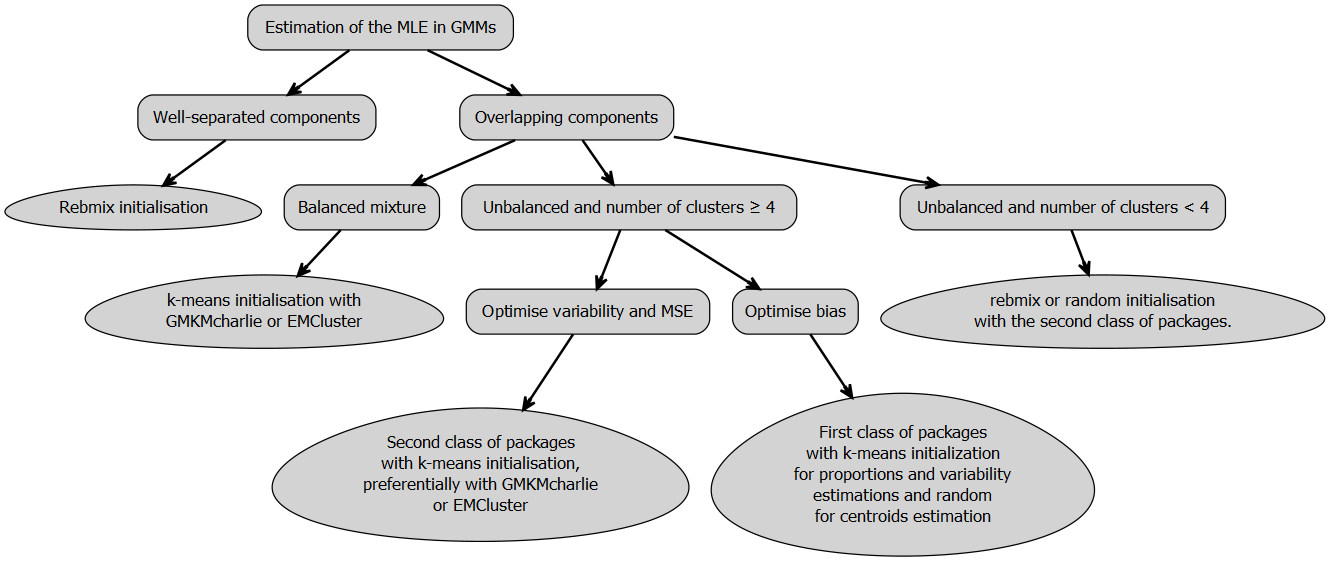
\includegraphics[width=1\linewidth]{./figures/decision_tree_GMMs} 

}

\caption{A decision tree to select the best combination of package and initialisation method with respect to the main characteristics of the mixture. It's worth pointing that in both univariate and low dimension multivariate settings, the recommandations are similar.}\label{fig:decision-tree-GMMs}
\end{figure}

Comparing all these packages suggest several improvements.

\begin{enumerate}
\def\labelenumi{\arabic{enumi}.}
\item
  The use of C++ code speeds up the convergence of the EM algorithm
  compared to a native R implementation.
\item
  All packages dealing with GMMs should use \emph{k}-means for overlapping, complex mixtures and rebmix initialisation for well-separated components, provided that the dimension of the dataset is relatively small. The final choice between these two could be set after a first run or visual inspection aiming at determining roughly the level of entropy across mixture proportions and the degree of overlap between components.
\item
  The packages should allow the user to set their own termination criteria (either relative or absolute log-likelihood or over the estimates after normalisation). Interestingly, \pkg{EMMIXmfa} is the only package among those examined that allows the user to consider an absolute or relative convergence endpoint of the EM algorithm, through the \texttt{conv\_measure} attribute, with \texttt{diff} and \texttt{ratio} options respectively.
\item
  With a great number of components or complex overlapping distributions, the optimal package should integrate prior information when available, e.g.~via Bayesian estimation.
\end{enumerate}

While \pkg{mclust} appeared as the most complete package to model GMMs in R, none of the packages reviewed in this report features all the characteristics mentioned above.
We thus strongly believe that our observations will help users identify the most suitable packages and parameters for their analyses and guide the development or updates of future packages.

\hypertarget{simulation-settings}{%
\section{Simulation settings}\label{simulation-settings}}

For ease of reading, we reproduce below the parameter configurations used to run the three benchmarks, respectively for the univariate (Table \ref{tab:parameter-configuration-univariate}), bivariate (\ref{tab:parameter-configuration-bivariate}) and high dimensional setting (Table \ref{tab:parameter-configuration-HD}).

\begin{table}[!h]

\caption{\label{tab:parameter-configuration-univariate}The 9 parameter configurations tested to generate the samples of the univariate experiment, with $k=4$ components.}
\centering
\resizebox{\linewidth}{!}{
\begin{tabular}[t]{cccccc}
\toprule
\textbf{ID} & \textbf{Entropy} & \textbf{OVL} & \textbf{Proportions} & \textbf{Means} & \textbf{Correlations}\\
\midrule
U1 & 1.00 & 3.3e-05 & 0.25 / 0.25 / 0.25 / 0.25 & 0 / 4 / 8 / 12 & 0.3 / 0.3 / 0.3 / 0.3\\
\midrule
U2 & 1.00 & 5.7e-03 & 0.25 / 0.25 / 0.25 / 0.25 & 0 / 4 / 8 / 12 & 1 / 1 / 1 / 1\\
\midrule
U3 & 1.00 & 2.0e-02 & 0.25 / 0.25 / 0.25 / 0.25 & 0 / 4 / 8 / 12 & 2 / 2 / 2 / 2\\
\midrule
U4 & 0.96 & 3.3e-05 & 0.2 / 0.4 / 0.2 / 0.2 & 0 / 4 / 8 / 12 & 0.3 / 0.3 / 0.3 / 0.3\\
\midrule
U5 & 0.96 & 5.8e-03 & 0.2 / 0.4 / 0.2 / 0.2 & 0 / 4 / 8 / 12 & 1 / 1 / 1 / 1\\
\midrule
\addlinespace
U6 & 0.96 & 2.0e-02 & 0.2 / 0.4 / 0.2 / 0.2 & 0 / 4 / 8 / 12 & 2 / 2 / 2 / 2\\
\midrule
U7 & 0.68 & 2.7e-05 & 0.1 / 0.7 / 0.1 / 0.1 & 0 / 4 / 8 / 12 & 0.3 / 0.3 / 0.3 / 0.3\\
\midrule
U8 & 0.68 & 4.4e-03 & 0.1 / 0.7 / 0.1 / 0.1 & 0 / 4 / 8 / 12 & 1 / 1 / 1 / 1\\
\midrule
U9 & 0.68 & 1.5e-02 & 0.1 / 0.7 / 0.1 / 0.1 & 0 / 4 / 8 / 12 & 2 / 2 / 2 / 2\\
\midrule
\bottomrule
\end{tabular}}
\end{table}

\begin{table}[!h]

\caption{\label{tab:parameter-configuration-bivariate}The 20 parameter configurations tested to generate the samples of the bivariate experiment.}
\centering
\resizebox{\linewidth}{!}{
\begin{tabular}[t]{cccccc}
\toprule
\textbf{ID} & \textbf{Entropy} & \textbf{OVL} & \textbf{Proportions} & \textbf{Means} & \textbf{Correlations}\\
\midrule
B1 & 1.00 & 0.15000 & 0.5 / 0.5 & (0,2);(2,0) & -0.8 / -0.8\\
\midrule
B2 & 1.00 & 0.07300 & 0.5 / 0.5 & (0,2);(2,0) & -0.8 / 0.8\\
\midrule
B3 & 1.00 & 0.07300 & 0.5 / 0.5 & (0,2);(2,0) & 0.8 / -0.8\\
\midrule
B4 & 1.00 & 0.00078 & 0.5 / 0.5 & (0,2);(2,0) & 0.8 / 0.8\\
\midrule
B5 & 1.00 & 0.07900 & 0.5 / 0.5 & (0,2);(2,0) & 0 / 0\\
\midrule
\addlinespace
B6 & 1.00 & 0.00000 & 0.5 / 0.5 & (0,20);(20,0) & -0.8 / -0.8\\
\midrule
B7 & 1.00 & 0.00000 & 0.5 / 0.5 & (0,20);(20,0) & -0.8 / 0.8\\
\midrule
B8 & 1.00 & 0.00000 & 0.5 / 0.5 & (0,20);(20,0) & 0.8 / -0.8\\
\midrule
B9 & 1.00 & 0.00000 & 0.5 / 0.5 & (0,20);(20,0) & 0.8 / 0.8\\
\midrule
B10 & 1.00 & 0.00000 & 0.5 / 0.5 & (0,20);(20,0) & 0 / 0\\
\midrule
\addlinespace
B11 & 0.47 & 0.06600 & 0.9 / 0.1 & (0,2);(2,0) & -0.8 / -0.8\\
\midrule
B12 & 0.47 & 0.01600 & 0.9 / 0.1 & (0,2);(2,0) & -0.8 / 0.8\\
\midrule
B13 & 0.47 & 0.05000 & 0.9 / 0.1 & (0,2);(2,0) & 0.8 / -0.8\\
\midrule
B14 & 0.47 & 0.00045 & 0.9 / 0.1 & (0,2);(2,0) & 0.8 / 0.8\\
\midrule
B15 & 0.47 & 0.03900 & 0.9 / 0.1 & (0,2);(2,0) & 0 / 0\\
\midrule
\addlinespace
B16 & 0.47 & 0.00000 & 0.9 / 0.1 & (0,20);(20,0) & -0.8 / -0.8\\
\midrule
B17 & 0.47 & 0.00000 & 0.9 / 0.1 & (0,20);(20,0) & -0.8 / 0.8\\
\midrule
B18 & 0.47 & 0.00000 & 0.9 / 0.1 & (0,20);(20,0) & 0.8 / -0.8\\
\midrule
B19 & 0.47 & 0.00000 & 0.9 / 0.1 & (0,20);(20,0) & 0.8 / 0.8\\
\midrule
B20 & 0.47 & 0.00000 & 0.9 / 0.1 & (0,20);(20,0) & 0 / 0\\
\midrule
\bottomrule
\end{tabular}}
\end{table}

\begin{table}[!h]

\caption{\label{tab:parameter-configuration-HD}The 16 parameter configurations tested to generate the samples in a high dimensional context. The first digit of each ID index refers
      to an unique parameter configuration (identified by its level of overlap, entropy and topological structure, either circular or ellipsoidal,
      of the covariance matrix, while the lowercase letter depicts the number of observations, a) with $n=200$ and b) with $n=2000$.}
\centering
\resizebox{\linewidth}{!}{
\begin{tabular}[t]{ccccc}
\toprule
\textbf{ID} & \textbf{OVL} & \textbf{\makecell[r]{Number of \\observations}} & \textbf{Proportions} & \textbf{Spherical}\\
\midrule
HD1a & 1e-04 & 200 & 0.5 / 0.5 & 
\includegraphics[scale=0.05]{figures/green_tick.png}\\
\midrule
HD1b & 1e-04 & 2000 & 0.5 / 0.5 & 
\includegraphics[scale=0.05]{figures/green_tick.png}\\
\midrule
HD2a & 1e-04 & 200 & 0.19 / 0.81 & 
\includegraphics[scale=0.05]{figures/green_tick.png}\\
\midrule
HD2b & 1e-04 & 2000 & 0.19 / 0.81 & 
\includegraphics[scale=0.05]{figures/green_tick.png}\\
\midrule
HD3a & 1e-04 & 200 & 0.5 / 0.5 & 
\includegraphics[scale=0.05]{figures/red_cross.png}\\
\midrule
\addlinespace
HD3b & 1e-04 & 2000 & 0.5 / 0.5 & 
\includegraphics[scale=0.05]{figures/red_cross.png}\\
\midrule
HD4a & 1e-04 & 200 & 0.21 / 0.79 & 
\includegraphics[scale=0.05]{figures/red_cross.png}\\
\midrule
HD4b & 1e-04 & 2000 & 0.21 / 0.79 & 
\includegraphics[scale=0.05]{figures/red_cross.png}\\
\midrule
HD5a & 2e-01 & 200 & 0.5 / 0.5 & 
\includegraphics[scale=0.05]{figures/green_tick.png}\\
\midrule
HD5b & 2e-01 & 2000 & 0.5 / 0.5 & 
\includegraphics[scale=0.05]{figures/green_tick.png}\\
\midrule
\addlinespace
HD6a & 2e-01 & 200 & 0.15 / 0.85 & 
\includegraphics[scale=0.05]{figures/green_tick.png}\\
\midrule
HD6b & 2e-01 & 2000 & 0.15 / 0.85 & 
\includegraphics[scale=0.05]{figures/green_tick.png}\\
\midrule
HD7a & 2e-01 & 200 & 0.5 / 0.5 & 
\includegraphics[scale=0.05]{figures/red_cross.png}\\
\midrule
HD7b & 2e-01 & 2000 & 0.5 / 0.5 & \includegraphics[scale=0.05]{figures/red_cross.png}\\
\midrule
HD8a & 2e-01 & 200 & 0.69 / 0.31 & \includegraphics[scale=0.05]{figures/red_cross.png}\\
\midrule
\addlinespace
HD8b & 2e-01 & 2000 & 0.69 / 0.31 & \includegraphics[scale=0.05]{figures/red_cross.png}\\
\midrule
\bottomrule
\end{tabular}}
\end{table}

\hypertarget{additional-files}{%
\section{Additional files}\label{additional-files}}

\begin{itemize}
\item
  Additional files related to the univariate setting

  \begin{itemize}
  \tightlist
  \item
    \textbf{S1.} Bootstrap distributions of the estimated parameters for each
    scenario described in \ref{tab:parameter-configuration-univariate}.
  \item
    \textbf{S2.} Mean, standard deviation, bias and MSE for each individually
    estimated parameter in configurations listed in \ref{tab:parameter-configuration-univariate}.
  \item
    \textbf{S3.} Distribution of the running times taken for the EM estimation of the parameters of the GMM, across all nine configurations described in \ref{tab:parameter-configuration-univariate}, for each benchmarked package. We selected the \emph{k}-means algorithm to initialise the EM algorithm, as being the least variable for a given package and scenario.
  \item
    \textbf{S4.} Distribution of the time computations taken by the six initialisation methods listed in Table \ref{tab:general-parameter-description-pdf}.
  \end{itemize}
\item
  Additional files related to the outliers setting:

  \begin{itemize}
  \tightlist
  \item
    \textbf{S5.} Bootstrap distributions of the estimated parameters used to
    generate Supplementary Figure 2. We additionally include the \pkg{otrimle} package, dedicated to these extreme distributions. Two configurations were tested, introducing \(2 \%\) and \(4 \%\) of outliers drawn from an improper uniform distribution.
  \item
    \textbf{S6.} Mean, standard deviation, bias and MSE for each individually
    estimated parameter in both configurations visualised on Supplementary Figure 2, for each combination of package and
    initialisation method.
  \end{itemize}
\item
  Additional files related to the bivariate benchmark:

  \begin{itemize}
  \item
    \textbf{S7.} Bootstrap distributions of the estimated parameters for each
    scenario described in \ref{tab:parameter-configuration-bivariate}.
  \item
    \textbf{S8.} Mean, standard deviation, bias and MSE for each individually
    estimated parameter in configurations listed in \ref{tab:parameter-configuration-bivariate}.
  \item
    \textbf{S9.} Distribution of the running times taken for the EM estimation of the parameters of the GMM, across all twenty configurations described in \ref{tab:parameter-configuration-bivariate}, for each benchmarked package. We selected the \emph{k}-means algorithm to initialise the EM algorithm, as being the least variable for a given package and scenario.
  \end{itemize}
\item
  Additional files related to the high-dimensional benchmark:

  \begin{itemize}
  \item
    \textbf{S10.} Bootstrap distributions of the estimated parameters for each
    scenario described in \ref{tab:parameter-configuration-HD}.
  \item
    \textbf{S11.} Mean, standard deviation, bias and MSE for each individually
    estimated parameter in configurations listed in \ref{tab:parameter-configuration-HD}.
  \item
    \textbf{S12.} Distribution of the running times taken for the EM estimation of the parameters of the GMM, across all twenty configurations described in \ref{tab:parameter-configuration-HD}, for each benchmarked package. We selected the \emph{k}-means algorithm to initialise the EM algorithm, as being the least variable for a given package and scenario.
  \end{itemize}
\end{itemize}

\hypertarget{references}{%
\section*{References}\label{references}}
\addcontentsline{toc}{section}{References}

\hypertarget{refs}{}
\begin{CSLReferences}{1}{0}
\leavevmode\vadjust pre{\hypertarget{ref-baek_etal10}{}}%
Baek, Jangsun, Geoffrey J. McLachlan, and Lloyd K. Flack. 2010. {``Mixtures of {Factor} {Analyzers} with {Common} {Factor} {Loadings}: {Applications} to the {Clustering} and {Visualization} of {High}-{Dimensional} {Data}.''} \emph{IEEE Transactions on Pattern Analysis and Machine Intelligence}. \url{https://doi.org/10.1109/TPAMI.2009.149}.

\leavevmode\vadjust pre{\hypertarget{ref-banfield_raftery93}{}}%
Banfield, Jeffrey D., and Adrian E. Raftery. 1993. {``Model-{Based Gaussian} and {Non-Gaussian Clustering}.''} \emph{Biometrics}. \url{https://doi.org/10.2307/2532201}.

\leavevmode\vadjust pre{\hypertarget{ref-R-HDclassif}{}}%
Berge, Laurent, Charles Bouveyron, and Stephane Girard. 2019. \emph{HDclassif: High Dimensional Supervised Classification and Clustering}.

\leavevmode\vadjust pre{\hypertarget{ref-biernacki_etal03}{}}%
Biernacki, Christophe, Gilles Celeux, and Gérard Govaert. 2003. {``Choosing Starting Values for the {EM} Algorithm for Getting the Highest Likelihood in Multivariate {Gaussian} Mixture Models.''} \emph{Computational Statistics \& Data Analysis}. \url{https://doi.org/10.1016/S0167-9473(02)00163-9}.

\leavevmode\vadjust pre{\hypertarget{ref-bouveyron_girard09}{}}%
Bouveyron, Charles, and Stéphane Girard. 2009. {``{Robust Supervised Classification} with {Mixture Models}: {Learning} from {Data} with {Uncertain Labels}.''} \emph{Pattern Recognition}. \url{https://doi.org/10.1016/j.patcog.2009.03.027}.

\leavevmode\vadjust pre{\hypertarget{ref-celeux_govaert92}{}}%
Celeux, Gilles, and Gérard Govaert. 1992. {``A Classification {EM} Algorithm for Clustering and Two Stochastic Versions.''} \emph{Computational Statistics \& Data Analysis}. \url{https://doi.org/10.1016/0167-9473(92)90042-E}.

\leavevmode\vadjust pre{\hypertarget{ref-chen16}{}}%
Chen, Jiahua. 2016. {``Consistency of the {MLE} Under Mixture Models.''} \url{https://doi.org/10.1214/16-STS578}.

\leavevmode\vadjust pre{\hypertarget{ref-cochran34}{}}%
Cochran, W. G. 1934. {``The Distribution of Quadratic Forms in a Normal System, with Applications to the Analysis of Covariance.''} \emph{Mathematical Proceedings of the Cambridge Philosophical Society}. \url{https://doi.org/10.1017/S0305004100016595}.

\leavevmode\vadjust pre{\hypertarget{ref-dempster_etal77}{}}%
Dempster, A. P., N. M. Laird, and D. B. Rubin. 1977. {``Maximum {Likelihood} from {Incomplete Data Via} the {\emph{EM}} {Algorithm}.''} \emph{Journal of the Royal Statistical Society}. \url{https://doi.org/10.1111/j.2517-6161.1977.tb01600.x}.

\leavevmode\vadjust pre{\hypertarget{ref-fraley98}{}}%
Fraley, Chris. 1998. {``Algorithms for {Model-Based Gaussian Hierarchical Clustering}.''} \emph{SIAM Journal on Scientific Computing}. \url{https://doi.org/10.1137/S1064827596311451}.

\leavevmode\vadjust pre{\hypertarget{ref-geary36}{}}%
Geary, R. C. 1936. {``The {Distribution} of "{Student}'s" {Ratio} for {Non-Normal Samples}.''} \emph{Supplement to the Journal of the Royal Statistical Society}. \url{https://doi.org/10.2307/2983669}.

\leavevmode\vadjust pre{\hypertarget{ref-jin_etal16}{}}%
Jin, Chi, Yuchen Zhang, Sivaraman Balakrishnan, et al. 2016. {``Local {Maxima} in the {Likelihood} of {Gaussian Mixture Models}: {Structural Results} and {Algorithmic Consequences}.''} Curran Associates, Inc. https://doi.org/\url{https://doi.org/10.48550/arXiv.1609.00978}.

\leavevmode\vadjust pre{\hypertarget{ref-koopman36}{}}%
Koopman, B. O. 1936. {``On {Distributions Admitting} a {Sufficient Statistic}.''} \emph{Transactions of the American Mathematical Society}. \url{https://doi.org/10.2307/1989758}.

\leavevmode\vadjust pre{\hypertarget{ref-kwedlo13}{}}%
Kwedlo, Wojciech. 2013. {``A {New Method} for {Random Initialization} of the {EM Algorithm} for {Multivariate Gaussian Mixture Learning}.''} In \emph{Proceedings of the {8th International Conference} on {Computer Recognition Systems CORES 2013}}, edited by Robert Burduk, Konrad Jackowski, Marek Kurzynski, Michał Wozniak, and Andrzej Zolnierek. Springer International Publishing. \url{https://doi.org/10.1007/978-3-319-00969-8/_8}.

\leavevmode\vadjust pre{\hypertarget{ref-leytham84}{}}%
Leytham, K. M. 1984. {``Maximum {Likelihood Estimates} for the {Parameters} of {Mixture Distributions}.''} \emph{Water Resources Research}. \url{https://doi.org/10.1029/WR020i007p00896}.

\leavevmode\vadjust pre{\hypertarget{ref-lourens_etal13}{}}%
Lourens, Spencer, Ying Zhang, Jeffrey D Long, et al. 2013. {``Bias in {Estimation} of a {Mixture} of {Normal Distributions}.''} \emph{Journal of Biometrics \& Biostatistics}. \url{https://doi.org/10.4172/2155-6180.1000179}.

\leavevmode\vadjust pre{\hypertarget{ref-mclachlan_peel00}{}}%
McLachlan, Geoffrey, and David Peel. 2000. \emph{Finite {Mixture Models}: {McLachlan}/{Finite Mixture Models}}. John Wiley \& Sons, Inc. \url{https://doi.org/10.1002/0471721182}.

\leavevmode\vadjust pre{\hypertarget{ref-R-MixSim}{}}%
Melnykov, Volodymyr, Wei-Chen Chen, and Ranjan Maitra. 2021. \emph{MixSim: Simulating Data to Study Performance of Clustering Algorithms}.

\leavevmode\vadjust pre{\hypertarget{ref-rebmix2015a}{}}%
Nagode, Marko. 2015. {``Finite Mixture Modeling via REBMIX.''} \emph{Journal of Algorithms and Optimization}.

\leavevmode\vadjust pre{\hypertarget{ref-R-rebmix}{}}%
---------. 2022. \emph{Rebmix: Finite Mixture Modeling, Clustering \& Classification}.

\leavevmode\vadjust pre{\hypertarget{ref-nityasuddhi_bohning03}{}}%
Nityasuddhi, Dechavudh, and Dankmar Böhning. 2003. {``Asymptotic Properties of the {EM} Algorithm Estimate for Normal Mixture Models with Component Specific Variances.''} \emph{Computational Statistics \& Data Analysis}. \url{https://doi.org/10.1016/S0167-9473(02)00176-7}.

\leavevmode\vadjust pre{\hypertarget{ref-rebmix2020b}{}}%
Panic, Branislav, Jernej Klemenc, and Marko Nagode. 2020. {``Improved Initialization of the EM Algorithm for Mixture Model Parameter Estimation.''} \emph{Mathematics}. \url{https://doi.org/10.3390/math8030373}.

\leavevmode\vadjust pre{\hypertarget{ref-R-core}{}}%
R Core Team. 2023. \emph{R: A Language and Environment for Statistical Computing}. Vienna, Austria: R Foundation for Statistical Computing. \url{https://www.R-project.org/}.

\leavevmode\vadjust pre{\hypertarget{ref-R-EMMIXmfa}{}}%
Rathnayake, Suren, Geoff McLachlan, David Peel, et al. 2019. \emph{EMMIXmfa: Mixture Models with Component-Wise Factor Analyzers}.

\leavevmode\vadjust pre{\hypertarget{ref-scrucca_raftery15}{}}%
Scrucca, Luca, and Adrian E. Raftery. 2015. {``Improved Initialisation of Model-Based Clustering Using {Gaussian} Hierarchical Partitions.''} \emph{Advances in Data Analysis and Classification}. \url{https://doi.org/10.1007/s11634-015-0220-z}.

\leavevmode\vadjust pre{\hypertarget{ref-shimizu_kaneko20}{}}%
Shimizu, Naoto, and Hiromasa Kaneko. 2020. {``Direct Inverse Analysis Based on {Gaussian} Mixture Regression for Multiple Objective Variables in Material Design.''} \emph{Materials \& Design}. \url{https://doi.org/10.1016/j.matdes.2020.109168}.

\leavevmode\vadjust pre{\hypertarget{ref-xu_knight10}{}}%
Xu, Dinghai, and John Knight. 2010. {``Continuous {Empirical Characteristic Function Estimation} of {Mixtures} of {Normal Parameters}.''} \emph{Econometric Reviews}. \url{https://doi.org/10.1080/07474938.2011.520565}.

\end{CSLReferences}


\address{%
Bastien Chassagnol\\
Laboratoire de Probabilités, Statistiques et Modélisation (LPSM), UMR
CNRS 8001\\%
4 Place Jussieu Sorbonne Université\\ 75005, Paris, France\\ \emph{ORCiD: \href{https://orcid.org/0000-0002-8955-2391}{0000-0002-8955-2391}}\\ \href{mailto:bastien_chassagnol@laposte.net}{\texttt{bastien\_chassagnol@laposte.net}}\\
%
%
%
%
}

\address{%
Antoine Bichat\\
Les Laboratoires Servier\\%
50 Rue Carnot\\ 92150, Suresnes, France\\ \url{https://rdrr.io/github/abichat/abutils/}\\ \emph{ORCiD: \href{https://orcid.org/0000-0001-6599-7081}{0000-0001-6599-7081}}\\ \href{mailto:antoine.bichat@servier.com}{\texttt{antoine.bichat@servier.com}}\\
%
%
%
%
}

\address{%
Cheïma Boudjeniba\\
Systems Biology Group, Dept. of Computational Biology, Institut
Pasteur\\%
25 Rue du Dr Roux\\ 75015 Paris\\ \href{mailto:cheima.boudjeniba@servier.com}{\texttt{cheima.boudjeniba@servier.com}}\\
%
%
%
%
}

\address{%
Pierre-Henri Wuillemin\\
Laboratoire d'Informatique de Paris 6 (LIP6), UMR 7606\\%
4 Place Jussieu Sorbonne Université\\ 75005, Paris, France\\ \url{http://www-desir.lip6.fr/~phw/}\\ \emph{ORCiD: \href{https://orcid.org/0000-0003-3691-4886}{0000-0003-3691-4886}}\\ \href{mailto:pierre-henri.wuillemin@lip6.fr}{\texttt{pierre-henri.wuillemin@lip6.fr}}\\
%
%
%
%
}

\address{%
Mickaël Guedj\\
Les Laboratoires Servier\\%
50 Rue Carnot\\ 92150, Suresnes, France\\ \url{https://michaelguedj.github.io/}\\ \emph{ORCiD: \href{https://orcid.org/0000-0001-6694-0554}{0000-0001-6694-0554}}\\ \href{mailto:mickael.guedj@gmail.com}{\texttt{mickael.guedj@gmail.com}}\\
%
%
%
%
}

\address{%
David Gohel\\
ArData\\%
59 rue Voltaire\\ 92800, PUTEAUX, France\\ \url{https://www.ardata.fr/expertise-r/}\\ \emph{ORCiD: \href{https://orcid.org/0000-0003-2837-8884}{0000-0003-2837-8884}}\\ \href{mailto:david.gohel@ardata.fr}{\texttt{david.gohel@ardata.fr}}\\
%
%
%
%
}

\address{%
Gregory Nuel\\
Laboratoire de Probabilités, Statistiques et Modélisation (LPSM), UMR
CNRS 8001\\%
4 Place Jussieu Sorbonne Université\\ 75005, Paris, France\\ \url{http://nuel.perso.math.cnrs.fr/}\\ \emph{ORCiD: \href{https://orcid.org/0000-0001-9910-2354}{0000-0001-9910-2354}}\\ \href{mailto:Gregory.Nuel@math.cnrs.fr}{\texttt{Gregory.Nuel@math.cnrs.fr}}\\
%
%
%
%
}

\address{%
Etienne Becht\\
Les Laboratoires Servier\\%
50 Rue Carnot\\ 92150, Suresnes, France\\ \emph{ORCiD: \href{https://orcid.org/0000-0003-1859-9202}{0000-0003-1859-9202}}\\ \href{mailto:etienne.becht@servier.com}{\texttt{etienne.becht@servier.com}}\\
%
%
%
%
}

\end{article}


\end{document}
